\documentclass[hidelinks,aspectratio=169]{beamer}
\usepackage[italian]{babel} 
\usepackage[utf8]{inputenc} 
\usepackage{fourier} 


%Slide colors
\usetheme{Boadilla}
\usecolortheme{beaver}

% Images
\usepackage{graphicx}
\usepackage{caption}
\usepackage{subcaption}
\usepackage{float}
\graphicspath{ {../Images} }

% FlowChart
\usepackage{smartdiagram}

% Stop hyphenation
\usepackage[none]{hyphenat}

% Coloring links
\usepackage{xcolor}

% License
\usepackage[
	type={CC},
	modifier={by-nc-sa},
	version={4.0},
]{doclicense}

% Command to enumerate frames title
\newcommand{\numcirc}[1]{%
	%   \usebeamerfont*{item projected}%
	\large
	\usebeamercolor[bg]{item projected}%
	\begin{pgfpicture}{-1ex}{0ex}{1ex}{2ex}
		\pgfpathcircle{\pgfpoint{0pt}{.75ex}}{1.2ex}
		\pgfusepath{fill}
		\pgftext[base]{\color{fg}#1}
	\end{pgfpicture}%
	\usebeamerfont*{frametitle}%
}

%Command to zoom in
\usepackage{mwe}
\makeatletter
\newsavebox\zb@x
\newcounter{z@@m}
\usepackage{calc}
\newdimen\B@r\newdimen\P@r
\newdimen\@zw\newdimen\@zh\newdimen\@zd

\newcommand{\zoombox}[2][0]{%
	\leavevmode%
	\sbox\zb@x{#2}%
	\setlength\B@r{1pt*\ratio{\wd\zb@x}{\ht\zb@x+\dp\zb@x}}%
	\setlength\P@r{1pt*\ratio{\paperwidth}{\paperheight}}%
	\ifdim\B@r>\P@r\relax%
	\setlength\@zw{\wd\zb@x}\setlength\@zh{\@zw*\ratio{\paperheight}{\paperwidth}}%
	\setlength\@zd{(\@zh-\ht\zb@x-\dp\zb@x)*\real{0.5}+\dp\zb@x}%
	\setlength\@zh{\@zh-\@zd}%
	\else%
	\setlength\@zh{\ht\zb@x+\dp\zb@x}%
	\setlength\@zw{\@zh*\ratio{\paperwidth}{\paperheight}}%
	\setlength\@zh{\ht\zb@x}\setlength\@zd{\dp\zb@x}%
	\fi%
	\makebox[0pt][l]{\makebox[\wd\zb@x][c]{\makebox[\@zw][l]{%
				\pdfdest name {zbfs\thez@@m} fitr
				width  \@zw\space
				height \@zh\space
				depth  \@zd\space
	}}}%
	\pdfdest name {zb\thez@@m} fitr
	width  \wd\zb@x\space
	height \ht\zb@x\space
	depth  \dp\zb@x\space
	\immediate\pdfannot 
	width  \wd\zb@x\space
	height \ht\zb@x\space
	depth  \dp\zb@x\space
	{%
		/Subtype/Link/H/N
		/Border [0 0 #1 [1 2]]
		/A <<
		/S/JavaScript
		/JS (
		if(typeof(zoomed)=='undefined'||!zoomed){
			var lastView=this.viewState;
			if(app.fs.isFullScreen) this.gotoNamedDest('zbfs\thez@@m');
			else this.gotoNamedDest('zb\thez@@m');
			zoomed=true;
		}else{
			this.viewState=lastView;
			zoomed=false;
		}
		)
		>>
	}%
	\usebox{\zb@x}%
	\stepcounter{z@@m}%
} 
\makeatother


%Header
\title[Tour guidato per bambini ai Musei Civici]{\textbf{Manuale per operatori\\Tour guidato per bambini ai Musei Civici}}
\author{Alice Balestieri\\Francesco Rombaldoni}
\date{}

\begin{document}
	
	%\frame\maketitle
	\begin{frame}
		\maketitle
		
		\vspace*{\fill}
		\centering
		\fboxrule=2pt
		\fbox
		{
			\begin{minipage}{0.9\linewidth}
				\small{Il seguente documento è ottimizzato per la visualizzazione digitale con \href{https://get.adobe.com/it/reader/}{\textcolor{blue}{Adobe~Acrobat~Reader}}.}  
			\end{minipage}
		}
	\end{frame}
	
	\begin{frame}
		Questa documentazione è un supporto volto a formare e facilitare gli Operatori Museali, nel far comprendere ai bambini le opere ed il contenuto degli spettacoli della Sonosfera(che sono visibili all'interno dei Musei Civici), attraverso un Tour Guidato da noi appositamente elaborato.
	\end{frame}
	
	\begin{frame}
		\small
		\tableofcontents
	\end{frame}
	
% Section here	
\section{Schema posizionamento delle Opere all'interno del Museo}
	
	\begin{frame}{Schema posizionamento delle Opere all'interno del Museo}
		\centering {\scalebox{0.67}{\begin{minipage}{\textwidth}
				
					\begin{center}
					\smartdiagramset{set color list={green!60!lime,red!80!black, blue!50!cyan, brown!80, violet!80}, back arrow disabled=true, module minimum width=10cm, module minimum height=1.5cm, module y sep=2.30, arrow line width=0.16cm, text width=8cm}
					\smartdiagram[flow diagram]{Scalone ingresso opera ceramica:\\ \textbf{La Medusa di Ferruccio Mengaroni}, Sala Giovanni Bellini: \\ \textbf{Opere di natura Ecclesiastica e provenienti dalla collezione Rossini}, Sala delle ceramiche collezione di Domenico Mazza: \\ \textbf{Piatto in ceramica con scoiattolo nero}, Sala arredi e sculture collezione Mosca, Sala natura e inganno}
				\end{center}
				
		\end{minipage}}}
	
	\end{frame}
	
	% Section here
	\section{Opere da mostrare all'interno del museo}
	
	\subsection{Mengaroni Ferruccio - Medusa}
	\begin{frame}{\numcirc{1} La Medusa di Ferruccio Mengaroni}
		\begin{itemize}
			\item La Medusa di Ferruccio Mengaroni, situata accanto allo scalone d'ingresso ai musei, sulla sinistra. È una delle opere più iconiche dei Musei Civici: si dice fosse avvolta da una temibile maledizione. L'imponente opera ceramica è stata ispirata, in parte, alle opere di Caravaggio, e al mito greco del mostro Medusa.\\
			L'artista realizzò l'opera prendendo come esempio la sua immagine in uno specchio, che ahimè, si ruppe e da lì in avanti la sciagura si abbatté su di lui. Durante il trasporto, in occasione dell'esposizione alla Biennale di Arti decorative di Monza, la monumentale opera si sbilanciò e Mengaroni, temendo che si rompesse, accorse a prenderla ma purtroppo venne schiacciato dal peso del suo stesso capolavoro.\par
		\end{itemize}
	\end{frame}
	
	\begin{frame}
		\begin{minipage}{\linewidth}
			\centering
			\zoombox{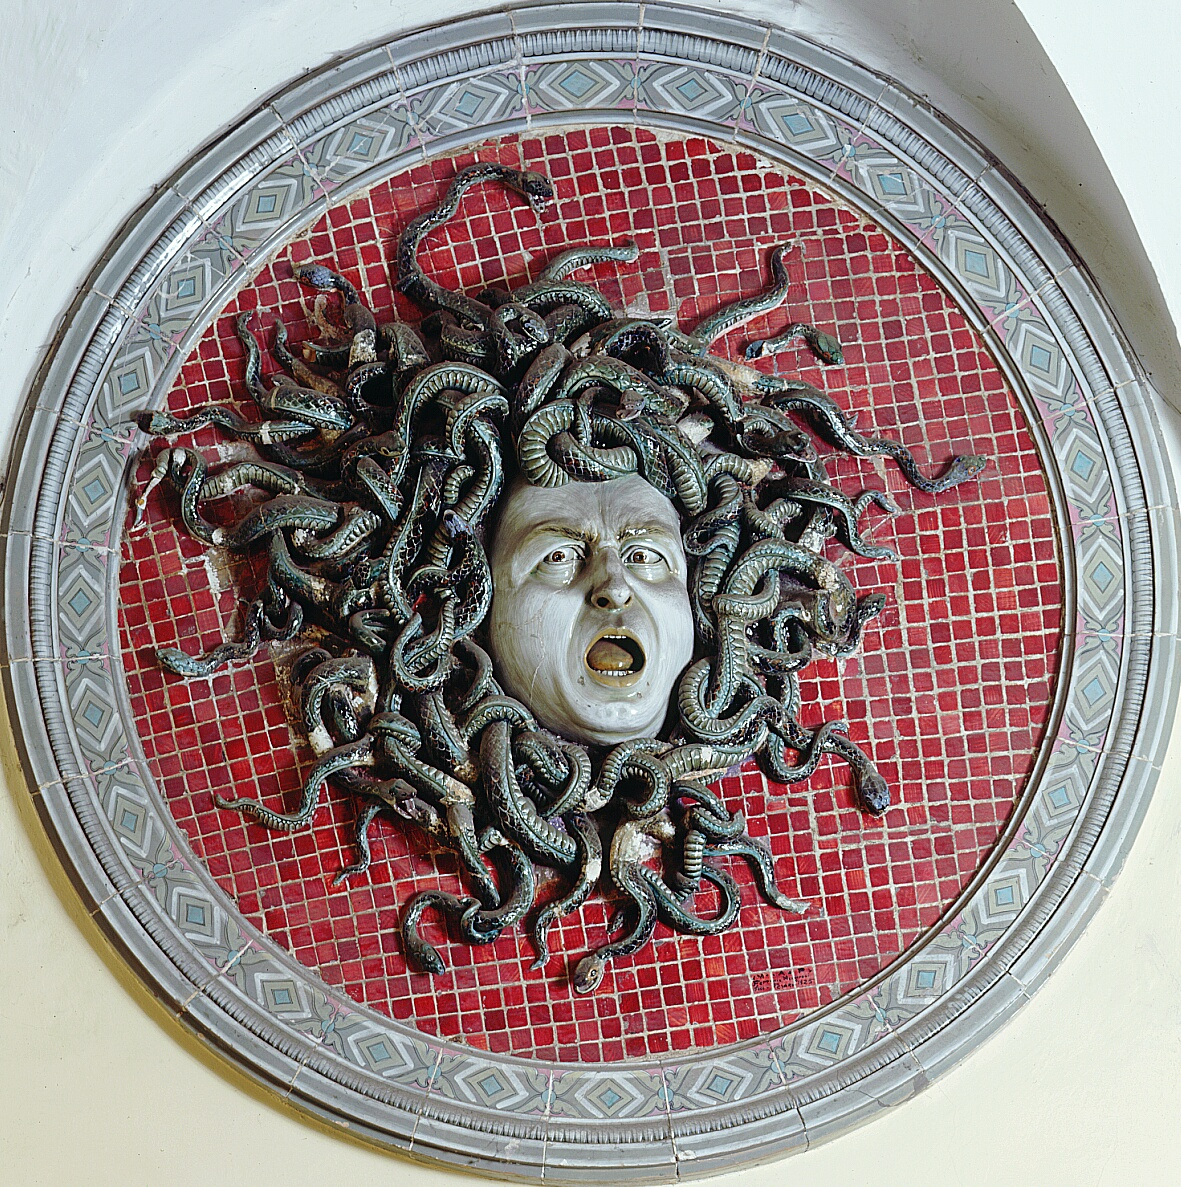
\includegraphics[scale=1.3]{Mengaroni_Ferruccio-Medusa.jpg}}
			\captionof{figure}{Mengaroni Ferruccio - Medusa.}
		\end{minipage}
	\end{frame}
	
	\subsection{Bellini Giovanni - Incoronazione della Vergine}
	\begin{frame}{\numcirc{2} Mostrare la Pala Bellini}
		\begin{itemize}
			\item La \textbf{Pala Bellini} (presente nella sala Bellini) è un'altra delle opere più importanti del museo. Questa opera fu realizzata su commissione a Venezia dall'artista Giovanni Bellini per essere esposta all'interno della Chiesa di S. Francesco a Pesaro e venne trasportata via mare, divisa in parti e poi riassemblata in loco.\\
			  Sottolineare il dettaglio della \bfseries{Colomba} \bfseries{(che rappresenta lo Spirito Santo)}, presente nel pannello centrale contenente la scena dell'Incoronazione della Vergine, che ha alle sue spalle, come sfondo, la celebre Rocca di Gradara; è altrettanto importante far notare il dettaglio del \bfseries{Drago} \textit{di S.Giorgio e il Drago}, presente in basso tra i sette riquadri della predella.\par
		\end{itemize}
	\end{frame}

	\begin{frame}
		\bigskip
			\begin{minipage}{\linewidth}
			\centering
			\zoombox{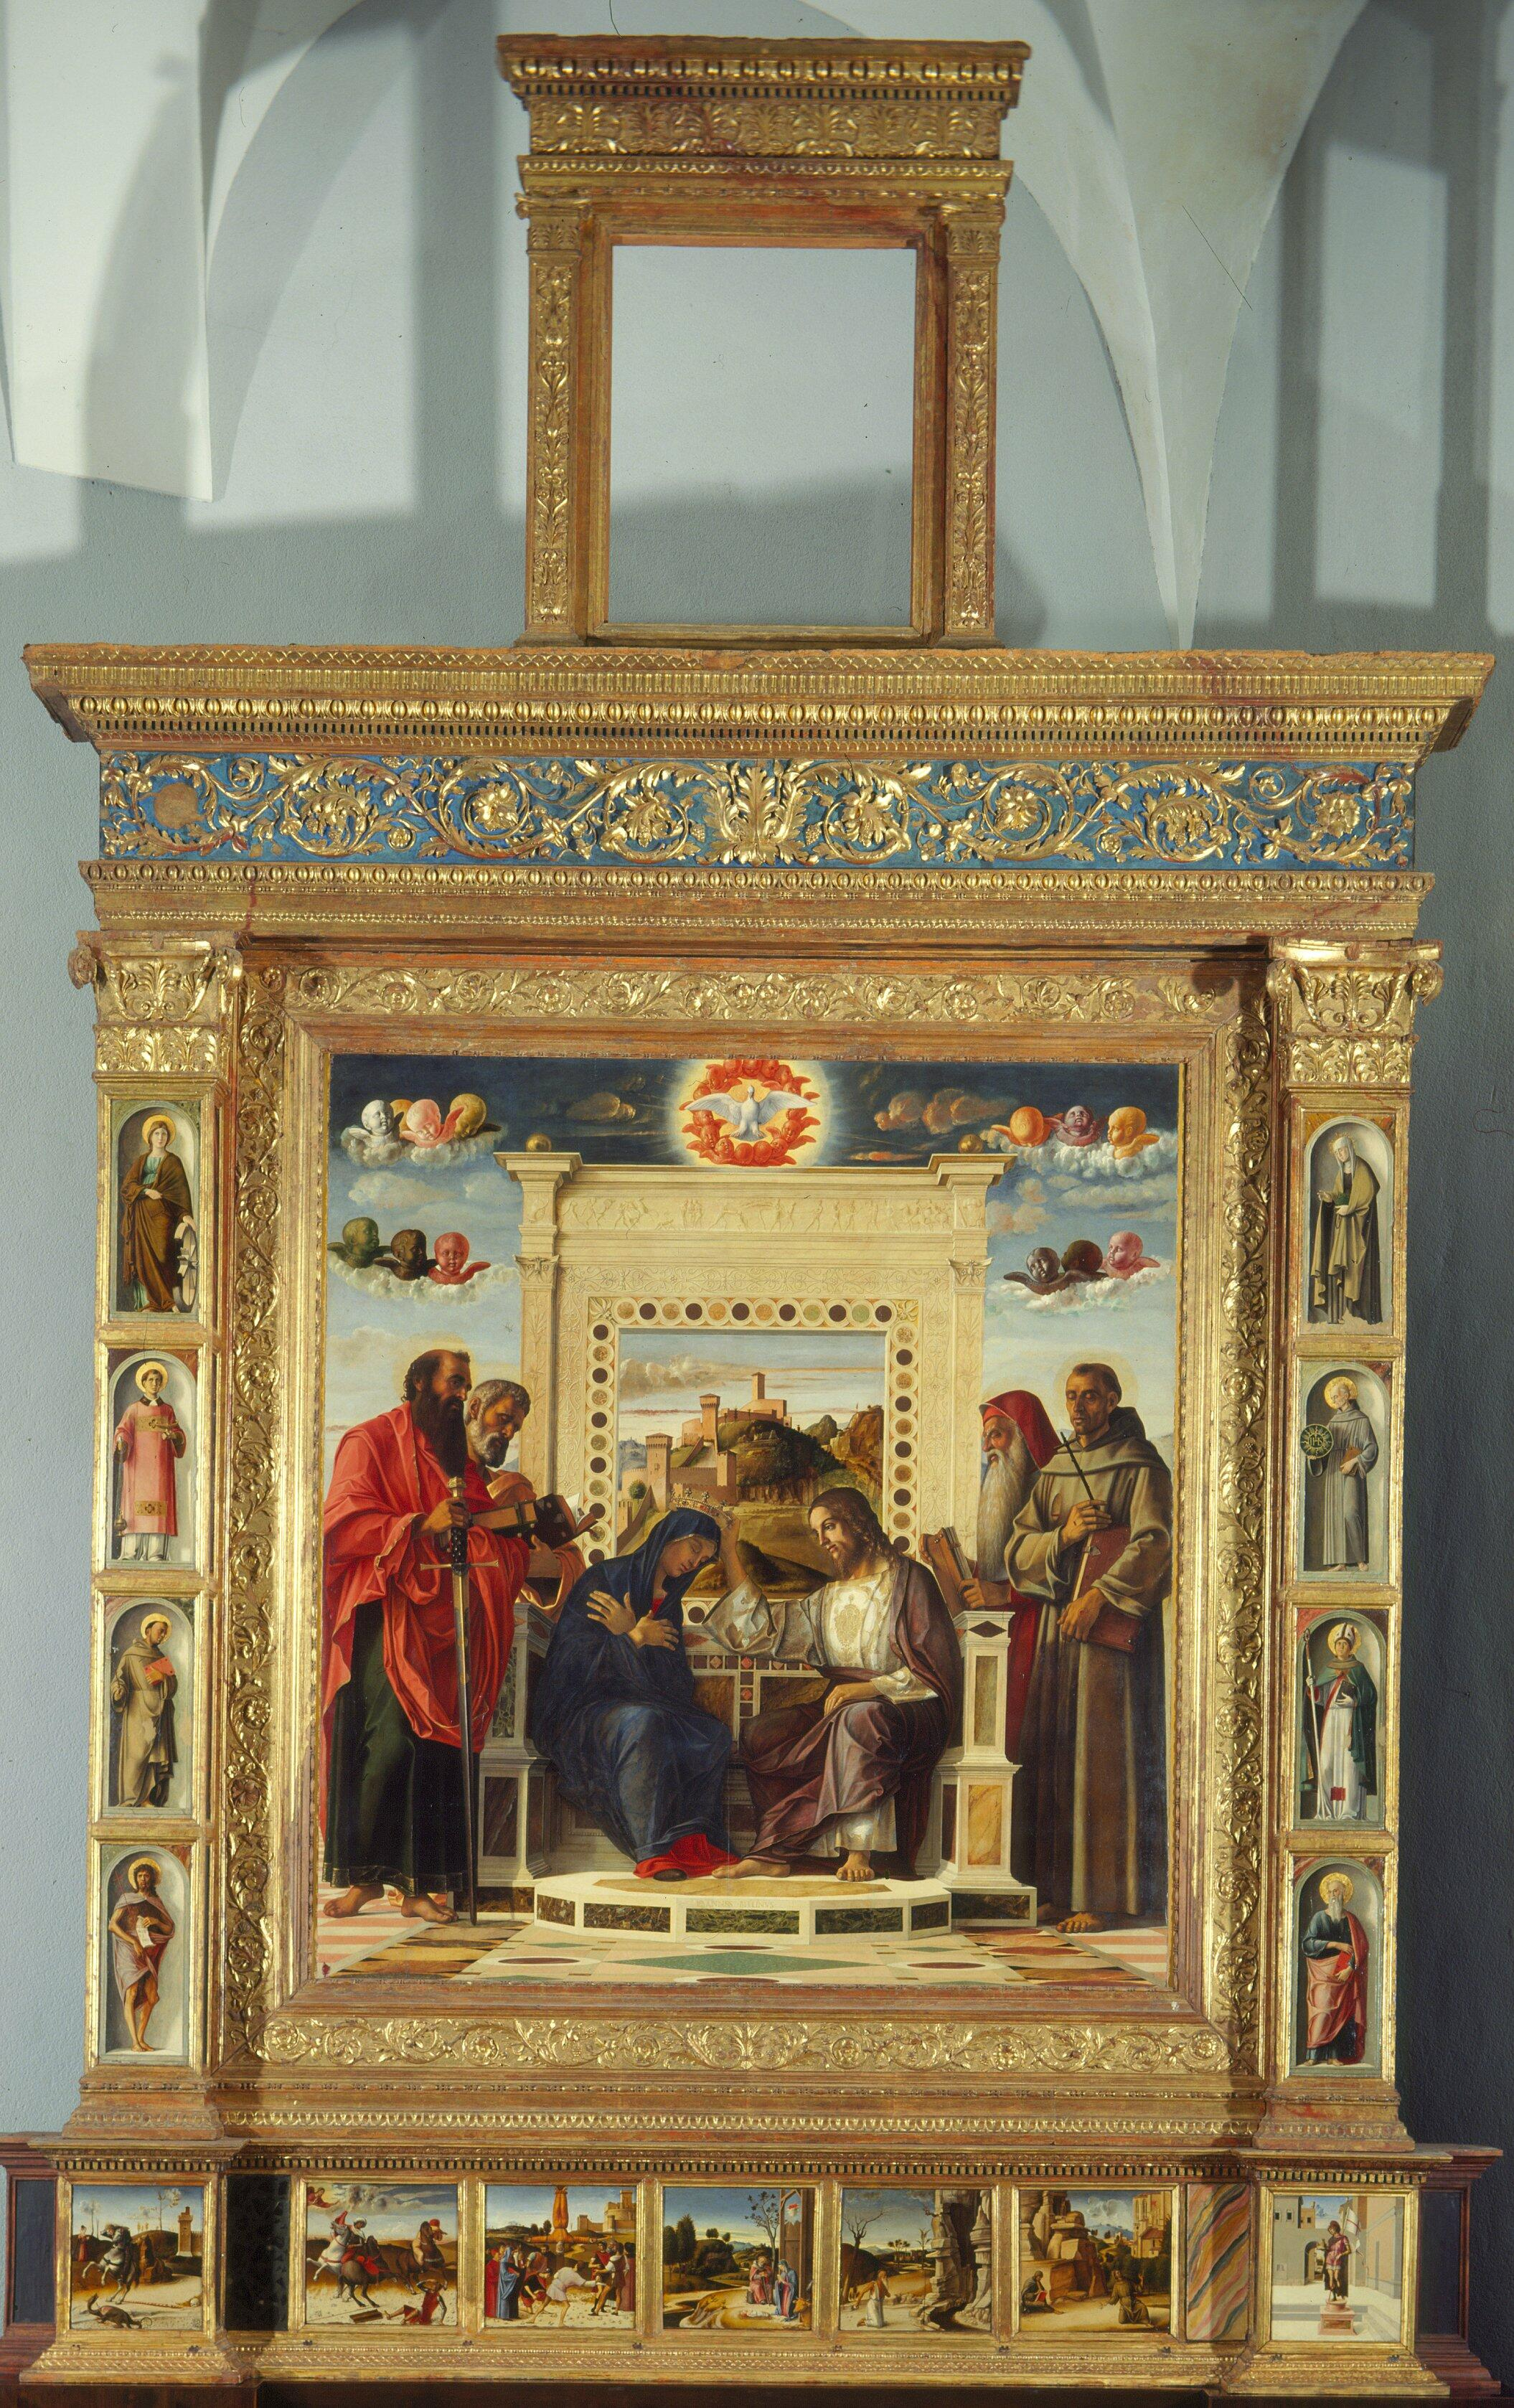
\includegraphics[scale=0.063]{Bellini_Giovanni-Incoronazione_della_Vergine.jpg}}
			\captionof{figure}{Bellini Giovanni - Incoronazione della Vergine.}
		\end{minipage}
	\end{frame}

	\begin{frame}
		\begin{minipage}{\linewidth}
			\centering
			\begin{minipage}{0.4\linewidth}
				\zoombox{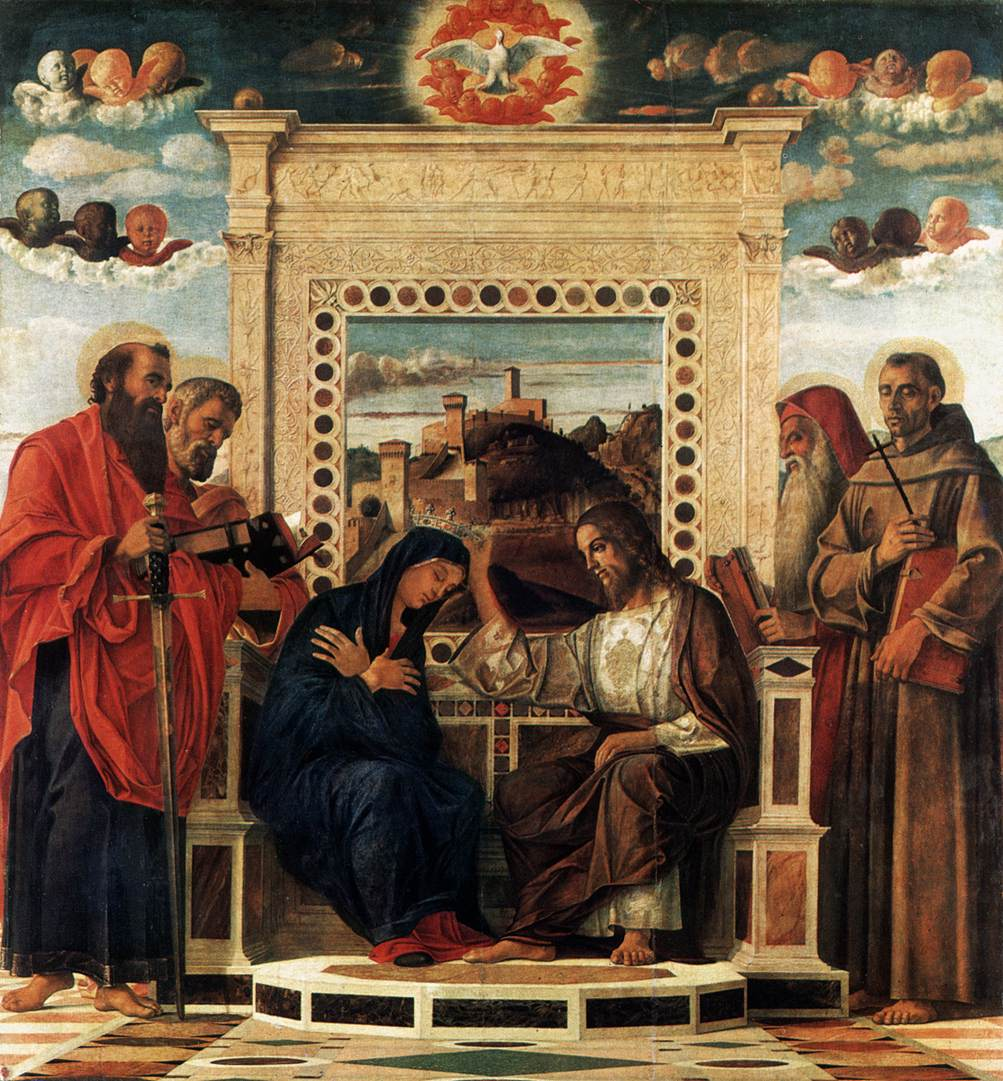
\includegraphics[scale=0.65]{Pala_di_pesaro_incoronazione.jpg}}
				\captionof{figure}{Dettaglio: Incoronazione della Vergine.}
			\end{minipage}
			\hfill
			\begin{minipage}{0.4\linewidth}
				\zoombox{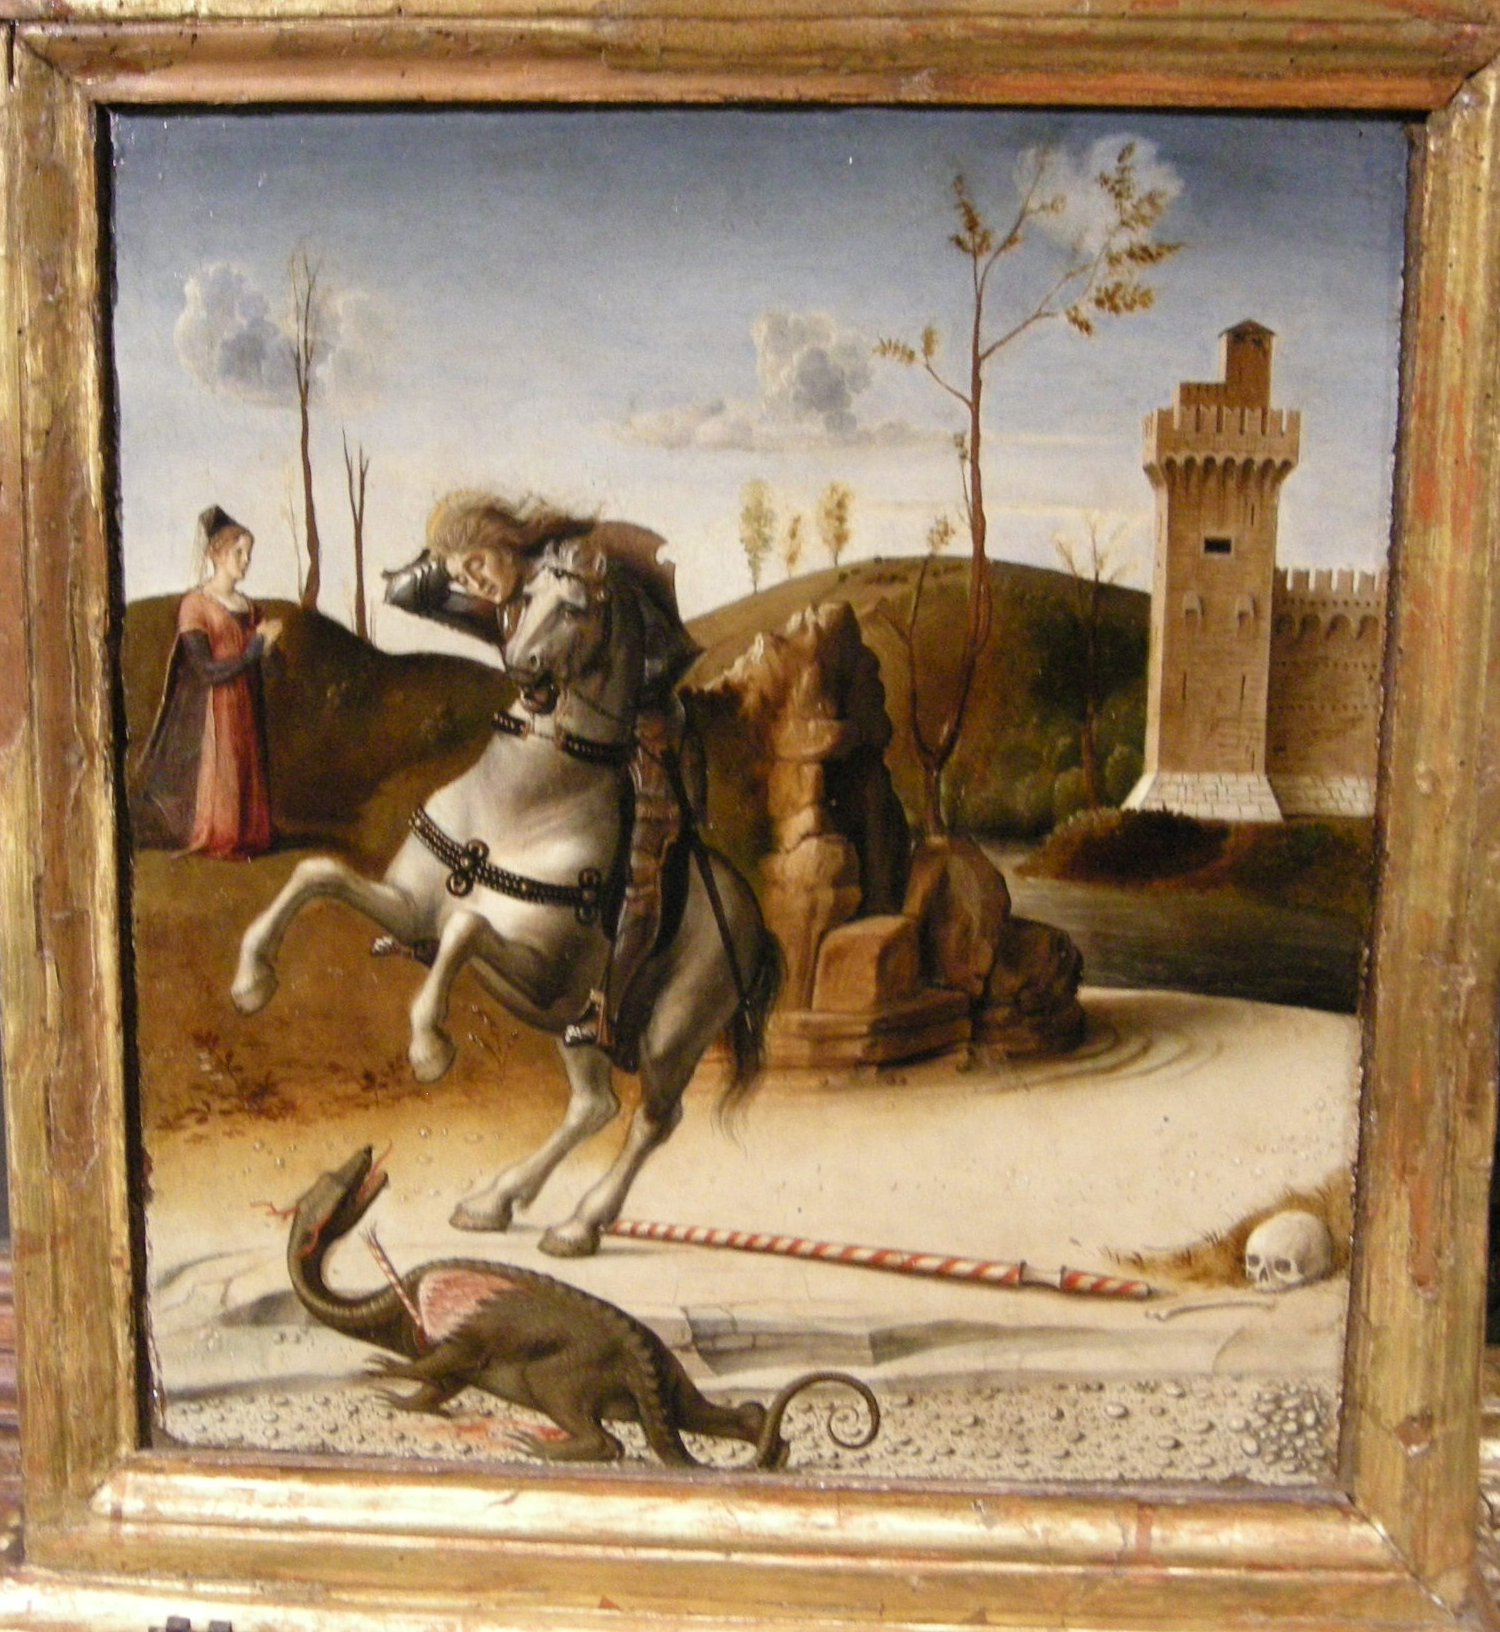
\includegraphics[scale=0.1]{Pala_di_Pesaro_S.Giorgio_e_il_Drago.jpg}}
				\captionof{figure}{Dettaglio: S. Giorgio e il Drago.}
			\end{minipage}
		\end{minipage}
	\end{frame}

	\subsection{Vitale da Bologna - Sant'Ambrogio in trono}
	\begin{frame}{\numcirc{3} Mostrare quadri che fanno più o meno uso della prospettiva}
		\begin{itemize}
			\item Mostrare quadri che fanno uso della prospettiva, confrontandoli con quelli che ne sono privi. \par 
		\end{itemize}
	\end{frame}

	\begin{frame}
		\bigskip
		\begin{minipage}{\linewidth}
			\centering
			\zoombox{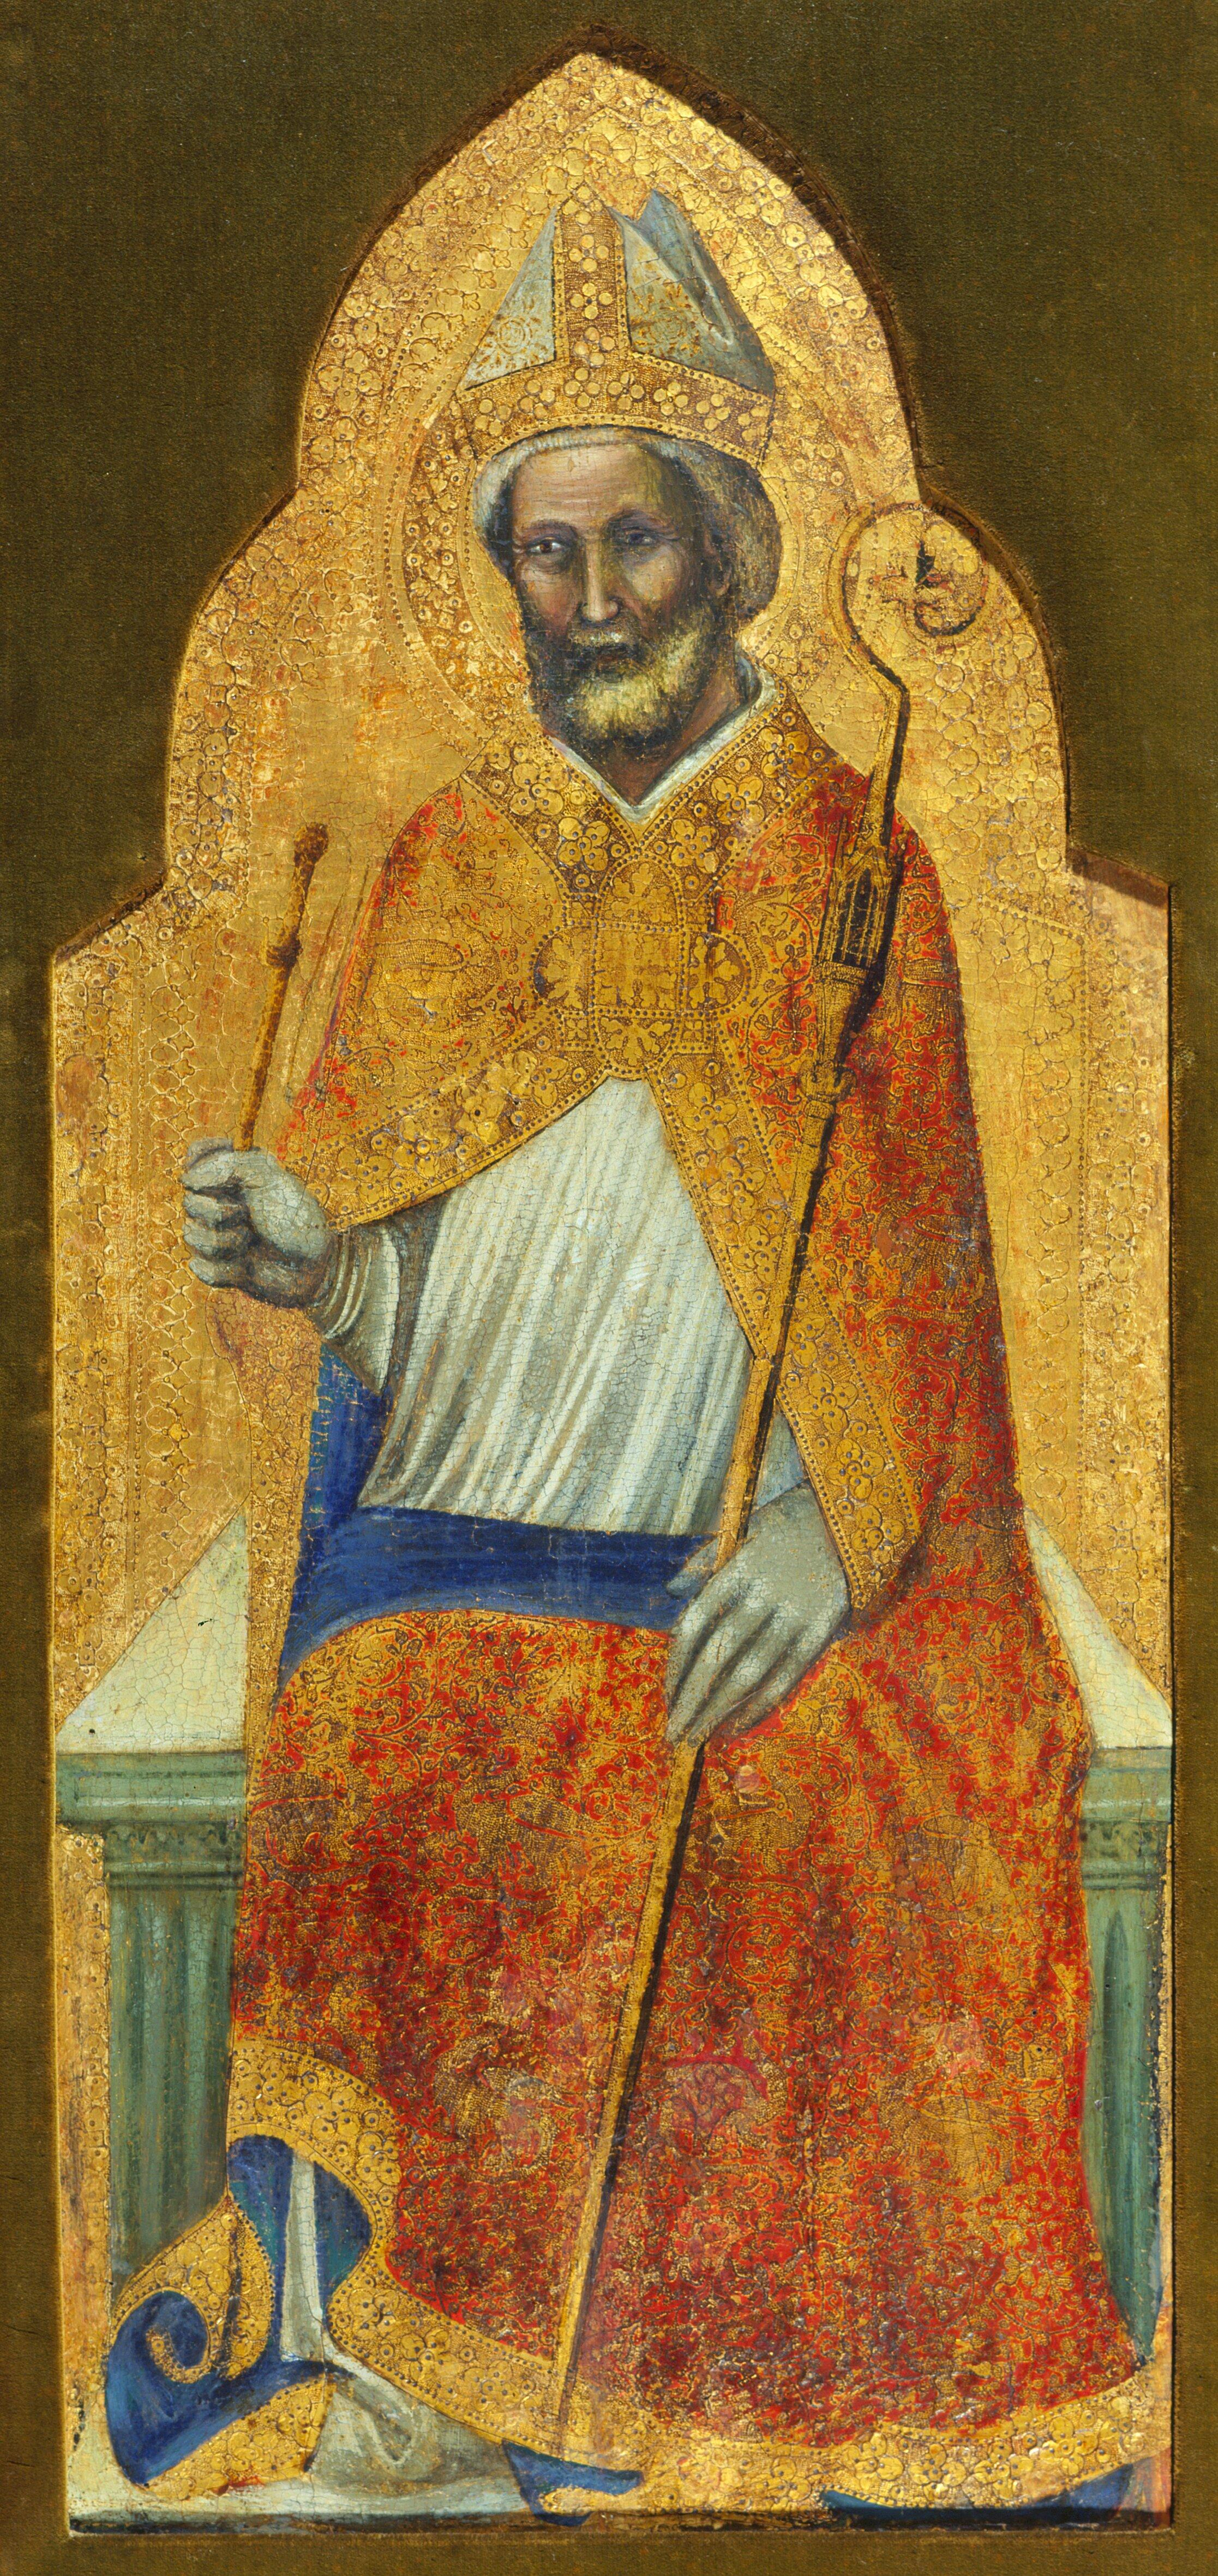
\includegraphics[scale=0.040]{Vitale_da_Bologna-Santo_Ambrogio_in_trono.jpg}}
			\captionsetup{justification=centering}
			\captionof{figure}{Vitale da Bologna - Sant'Ambrogio in trono. \\ Esempio di quadro privo di prospettiva parte della Collezione Rossini.}
		\end{minipage} 
	\end{frame}

	\subsection{Desani Pietro - Rebecca ed Eleazar}
	\begin{frame}{\numcirc{4} Esporre gli elementi che contraddistinguono la Collezione Rossini}
		\begin{itemize}
			\item Spiegare gli elementi che contraddistinguono la scelta delle opere, da parte di Rossini, da annettere alla sua collezione: come il \textbf{Rosso vermiglio}, \textbf{l'oro ed i gioielli} nei dipinti e ricordare ai visitatori che quello sfarzo era in realtà in contrasto con le sue umili origini ed erano da lui apprezzate proprio per mostrare alle dame ed ai nobili dell'epoca era riuscito ad arrivare con il suo talento. \par
		\end{itemize}
	\end{frame}
	
	\begin{frame}
		\begin{minipage}{\linewidth}
			\centering
			\zoombox{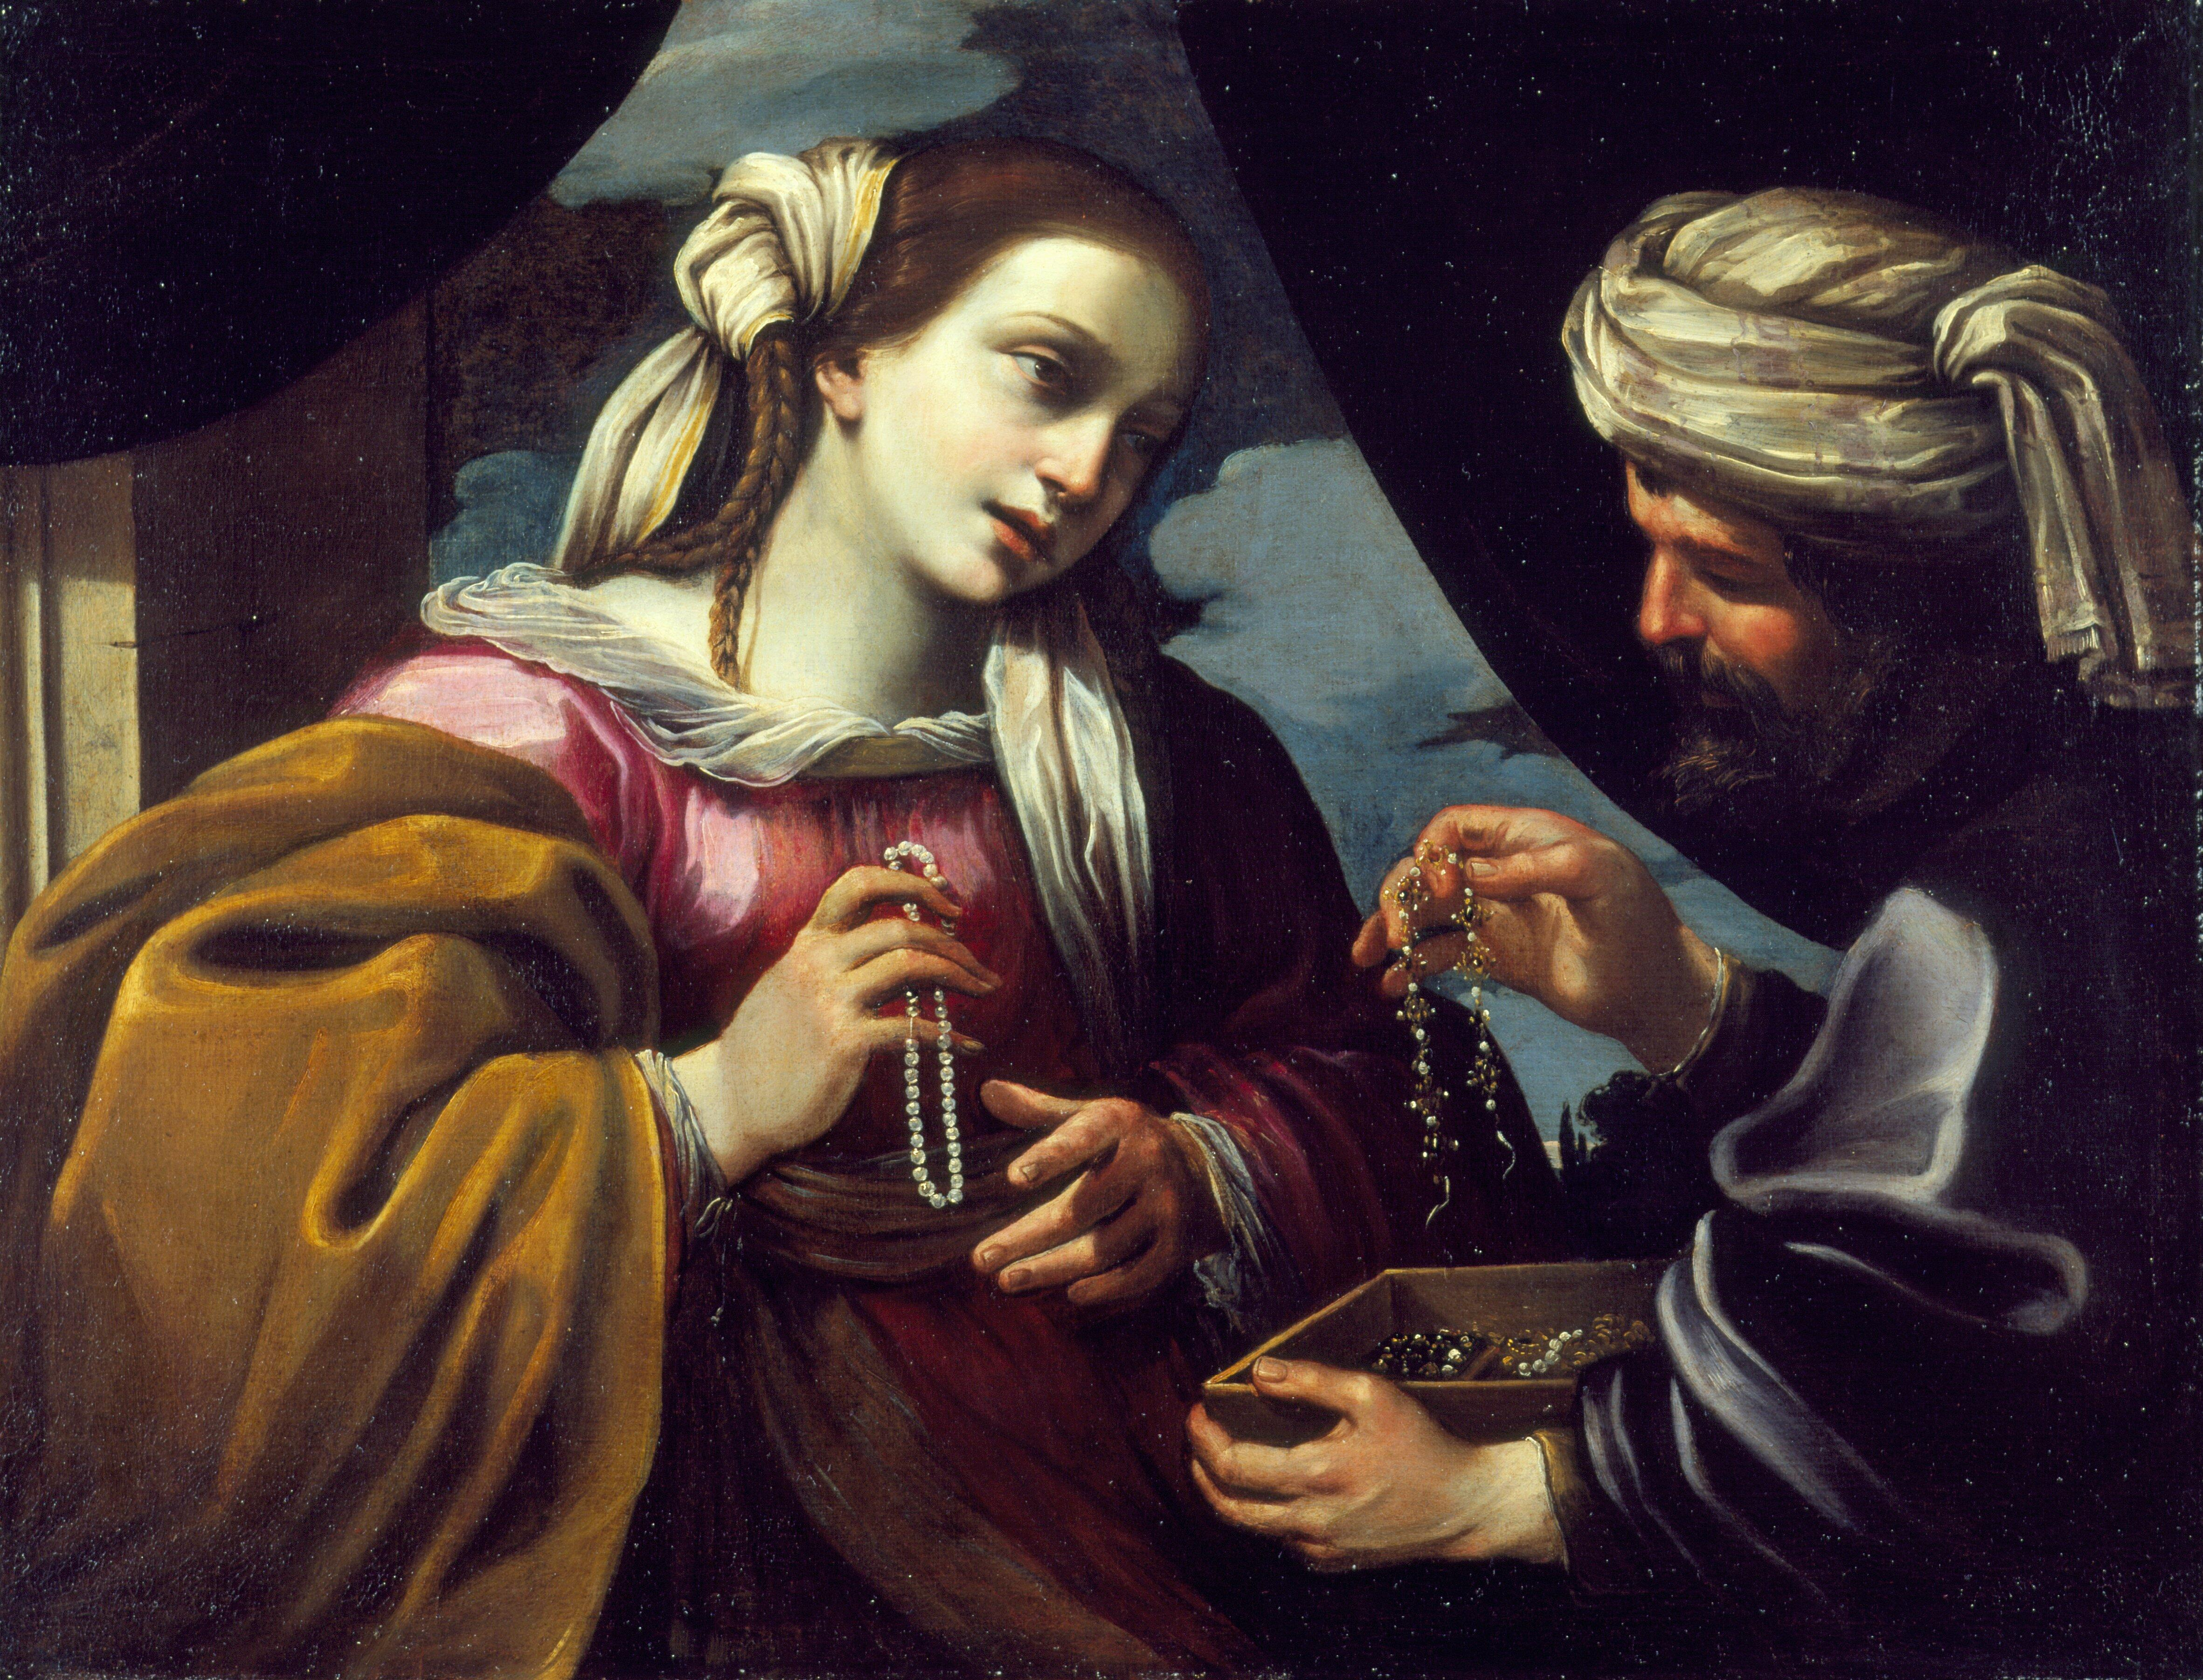
\includegraphics[scale = 0.05]{Desani_Pietro-Rebecca_ed_Eleazar.jpg}}
			\captionof{figure}{Desani Pietro - Rebecca ed Eleazar.}
		\end{minipage}
	\end{frame}

	\subsection{Leda e il Cigno (Giove) di fattura ad opera di Giovanni Antonio Garella}
	\begin{frame}{\numcirc{5} Illustrare il piatto dove è presente lo scoiattolo nero}
		\begin{itemize}
			\item Accompagnare i bambini alla scoperta delle opere ceramiche come Leda e il Cigno, \textbf{ceramica della collezione Mazza} dove è presente lo \textbf{scoiattolo dall'insolito colore nero come appariva cinquecento anni fa}.\par \bigskip
			\begin{minipage}{\linewidth}
				\centering
				\zoombox{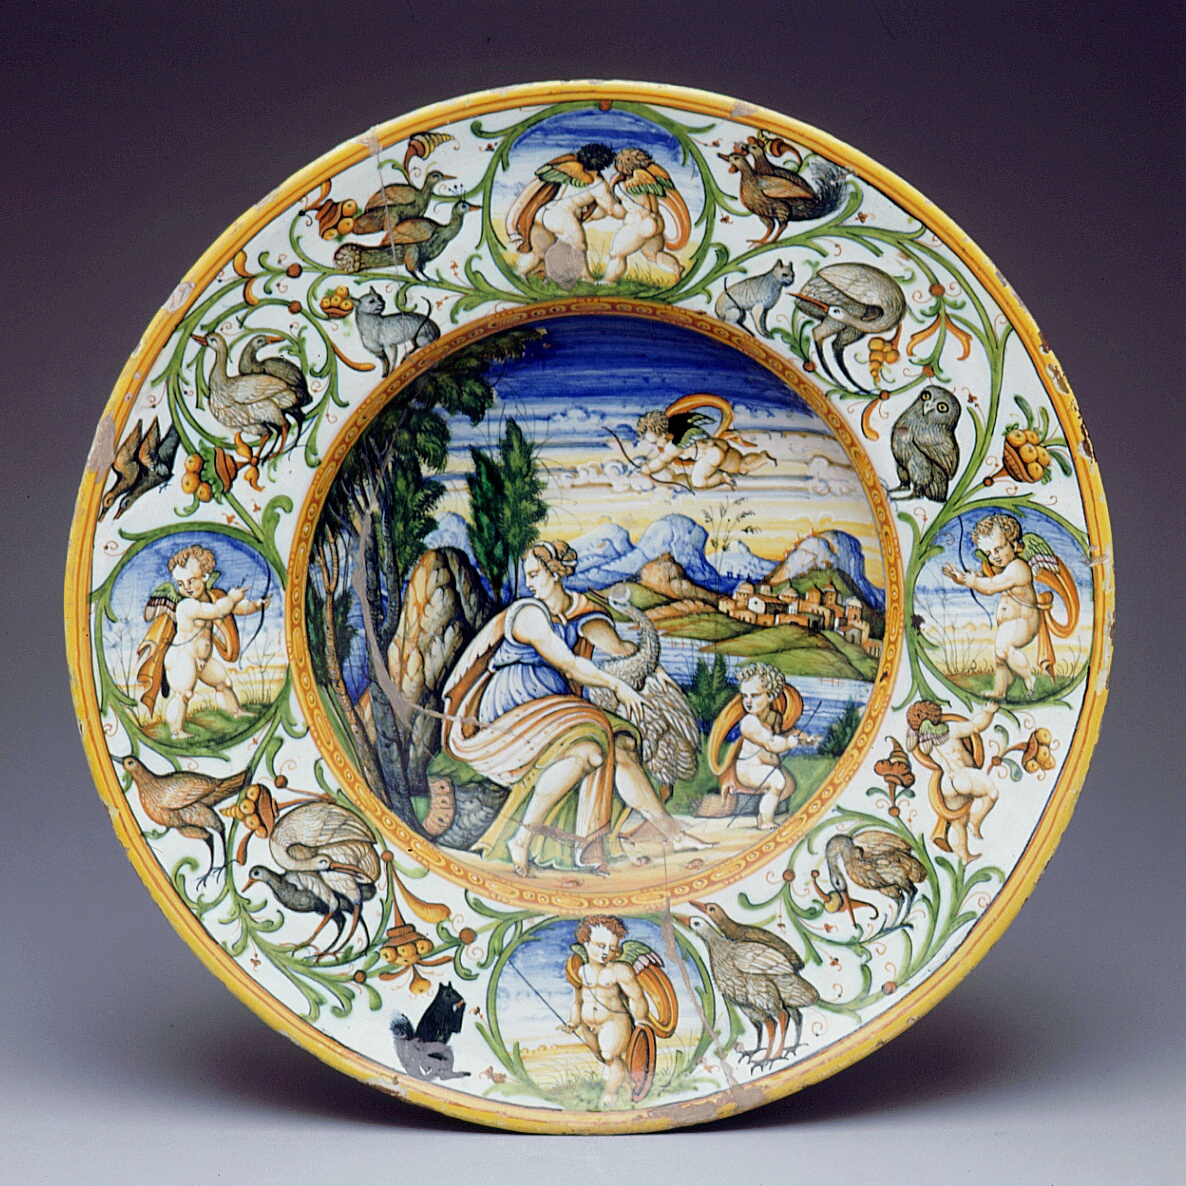
\includegraphics[scale=0.8]{Giovanni_Antonio_Garella-Leda_e_il_cigno.jpg}}
				\captionof{figure}{Leda e il Cigno (Giove) di fattura ad opera di Giovanni Antonio Garella.}
			\end{minipage}
		\end{itemize}
	\end{frame}
	
	\subsection{Specchio in vetro di Murano}
	\subsection{Oggetti in avorio e madreperla}
	\subsection{Vedute di Roma}
	\subsection{Orologio notturno}
	\begin{frame}{\numcirc{6} Far osservare con attenzione il pregiato specchio in vetro di Murano, gli oggetti in avorio e madreperla, lo stipo con vedute di Roma e l'orologio notturno}
		\begin{itemize}
			\item Far visionare, nella \textbf{Collezione Mosca}, il pregiato \textit{specchio in vetro di Murano} decorato con \textbf{incisioni d'uva d'argento nella parte interna e nella cornice di vetro da fiori}; gli \textbf{oggetti in avorio e madreperla}; lo \textit{Stipo con vedute di Roma} sottolineando come queste volessero essere una sorta di \textbf{cartoline} di Roma da mostrare ai commensali e l'\textit{Orologio Notturno}, usato dalla marchesa Toschi Mosca per comprendere che ore fossero quando si svegliava in preda all'insonnia.\par
		\end{itemize}
	\end{frame}

	\begin{frame}
		\bigskip
		\begin{minipage}{\linewidth}
			\centering
			\begin{minipage}{0.4\linewidth}
				\zoombox{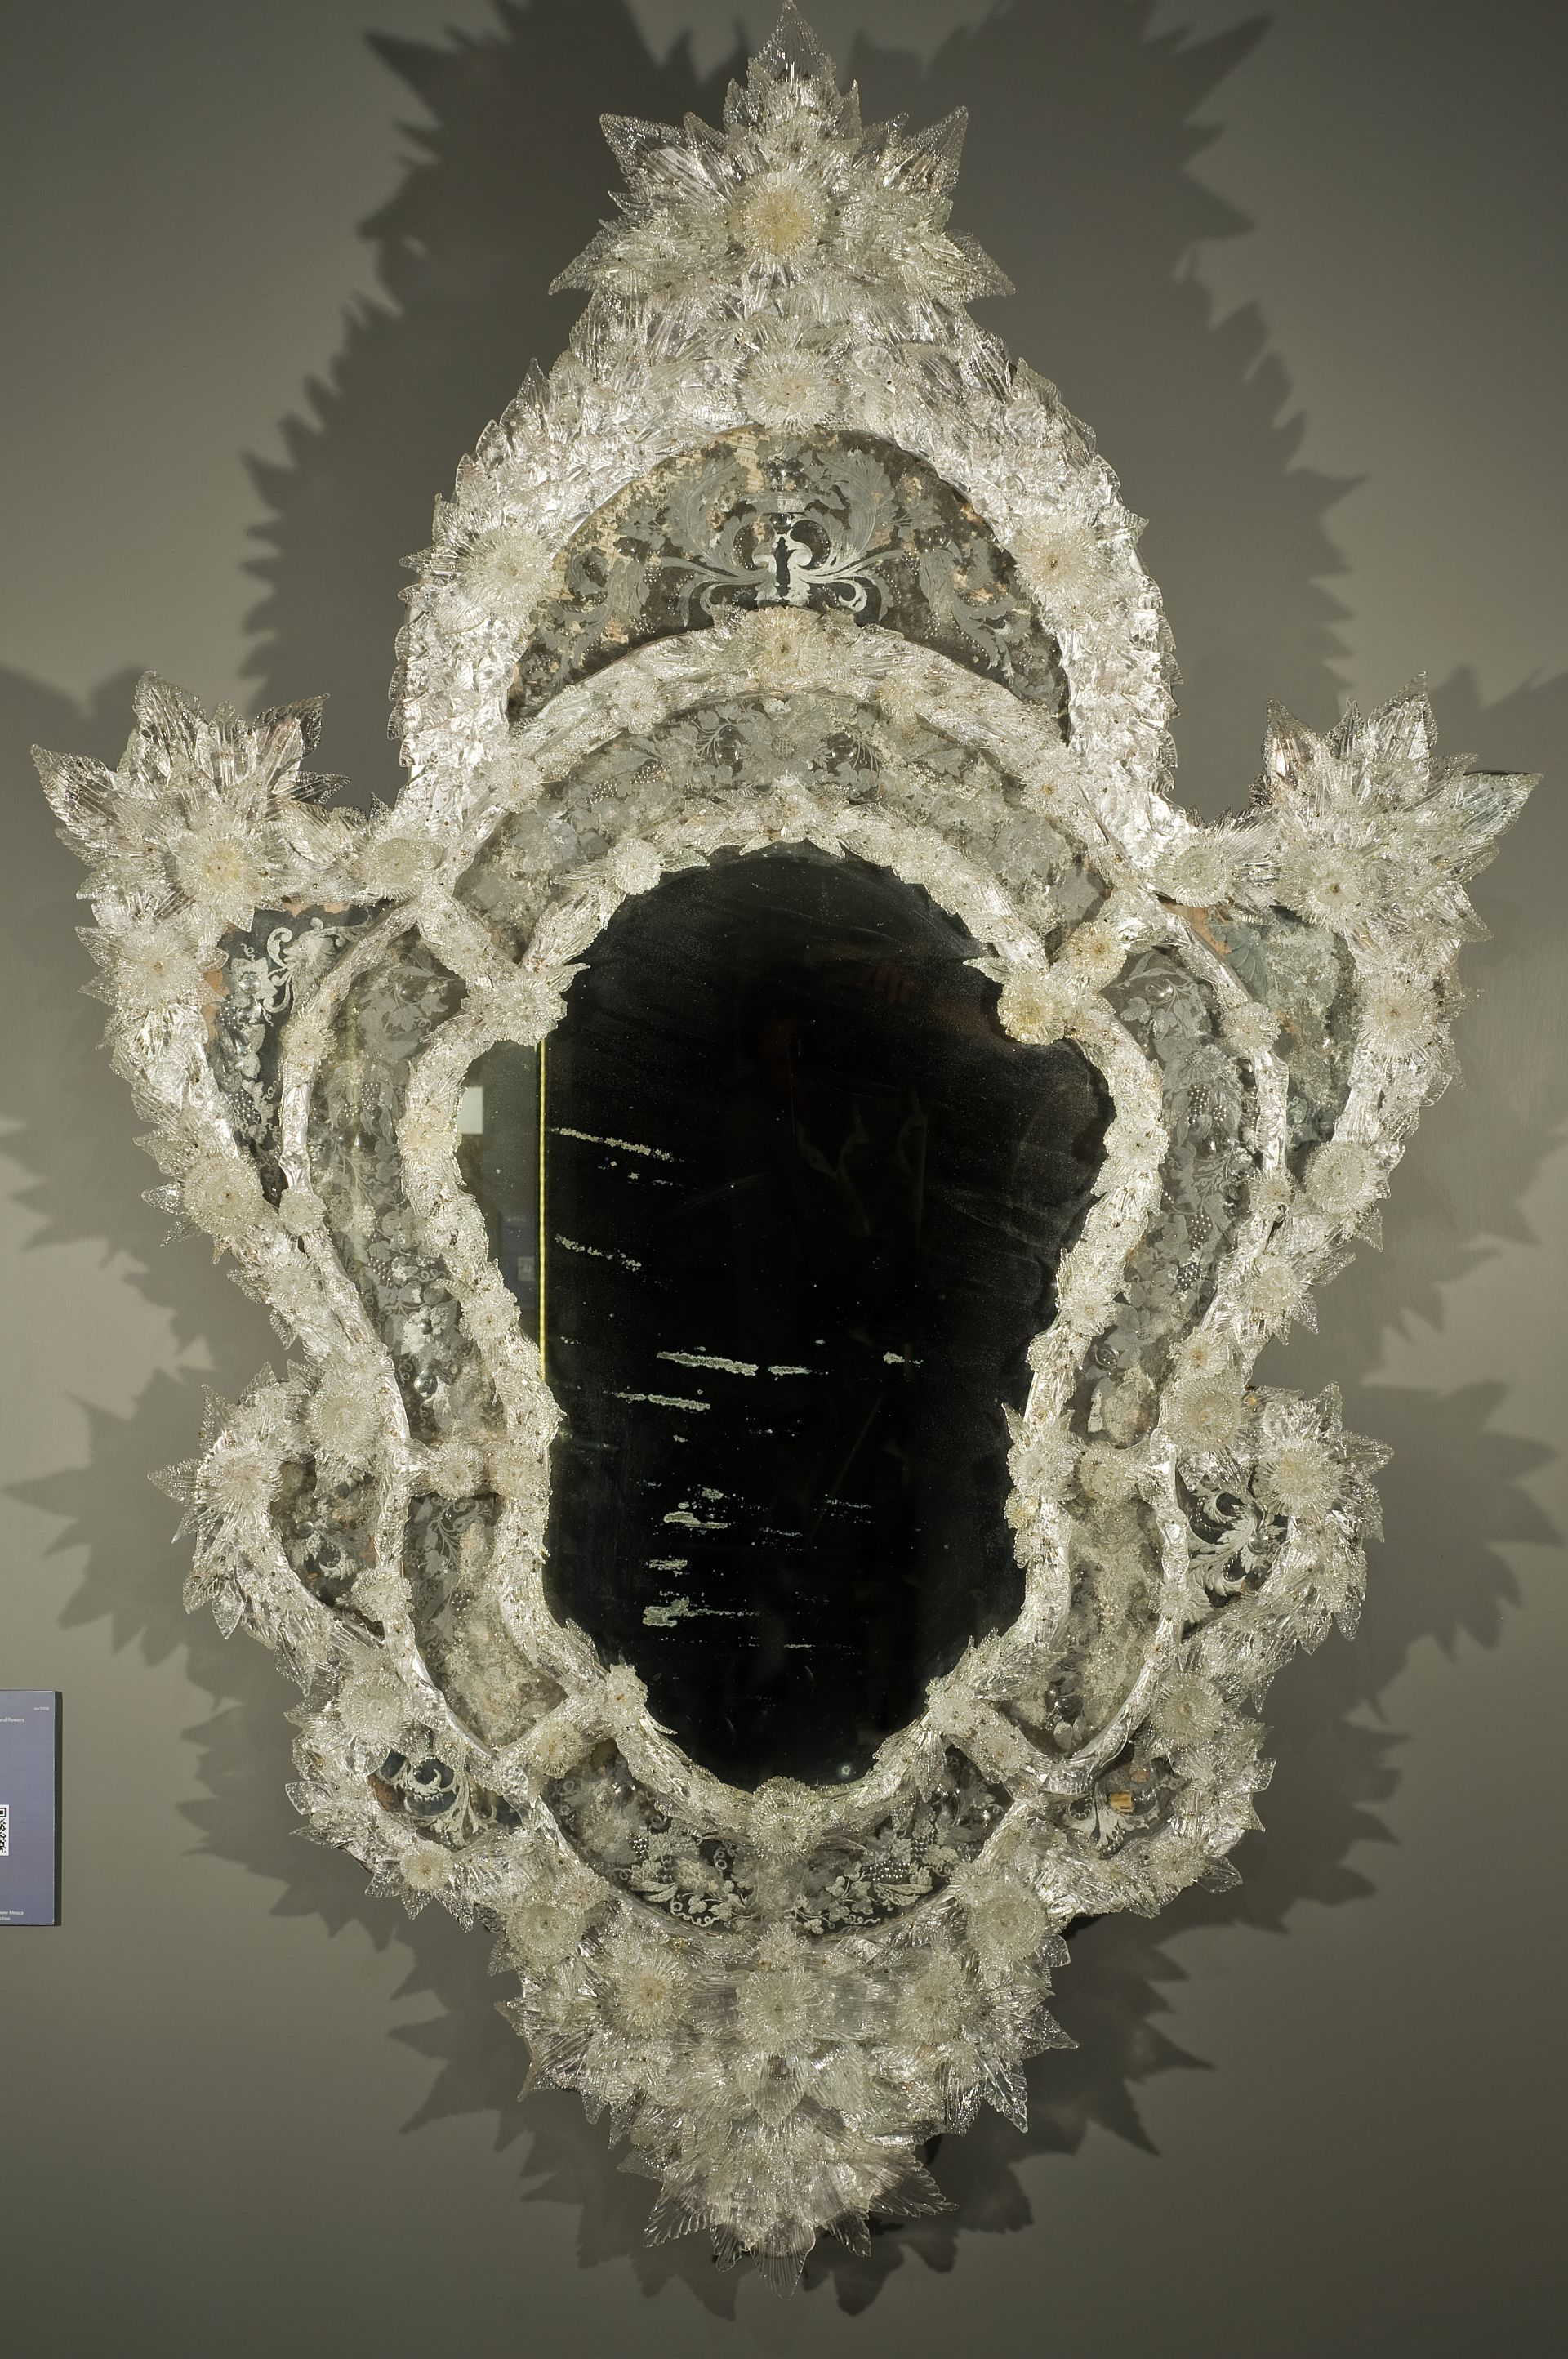
\includegraphics[scale=0.23]{Specchio_di_Murano.jpg}}
				\captionof{figure}{Specchio in vetro di Murano.}
			\end{minipage}
			\hfill
			\begin{minipage}{0.4\linewidth}
				\zoombox{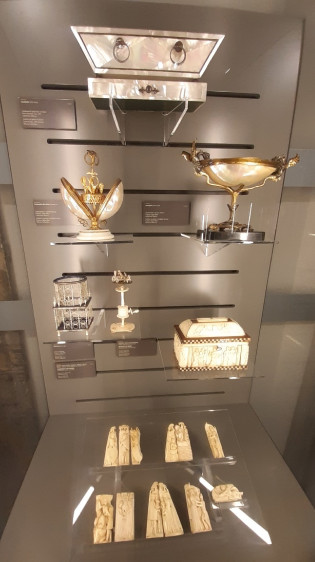
\includegraphics[scale=1.45]{Avorio_madreperla.jpg}}
				\captionof{figure}{Oggetti in avorio e madreperla.}
			\end{minipage}
		\end{minipage}
	\end{frame}

	\begin{frame}
		\bigskip
		\begin{minipage}{\linewidth}
			\centering
			\begin{minipage}{0.4\linewidth}
				\zoombox{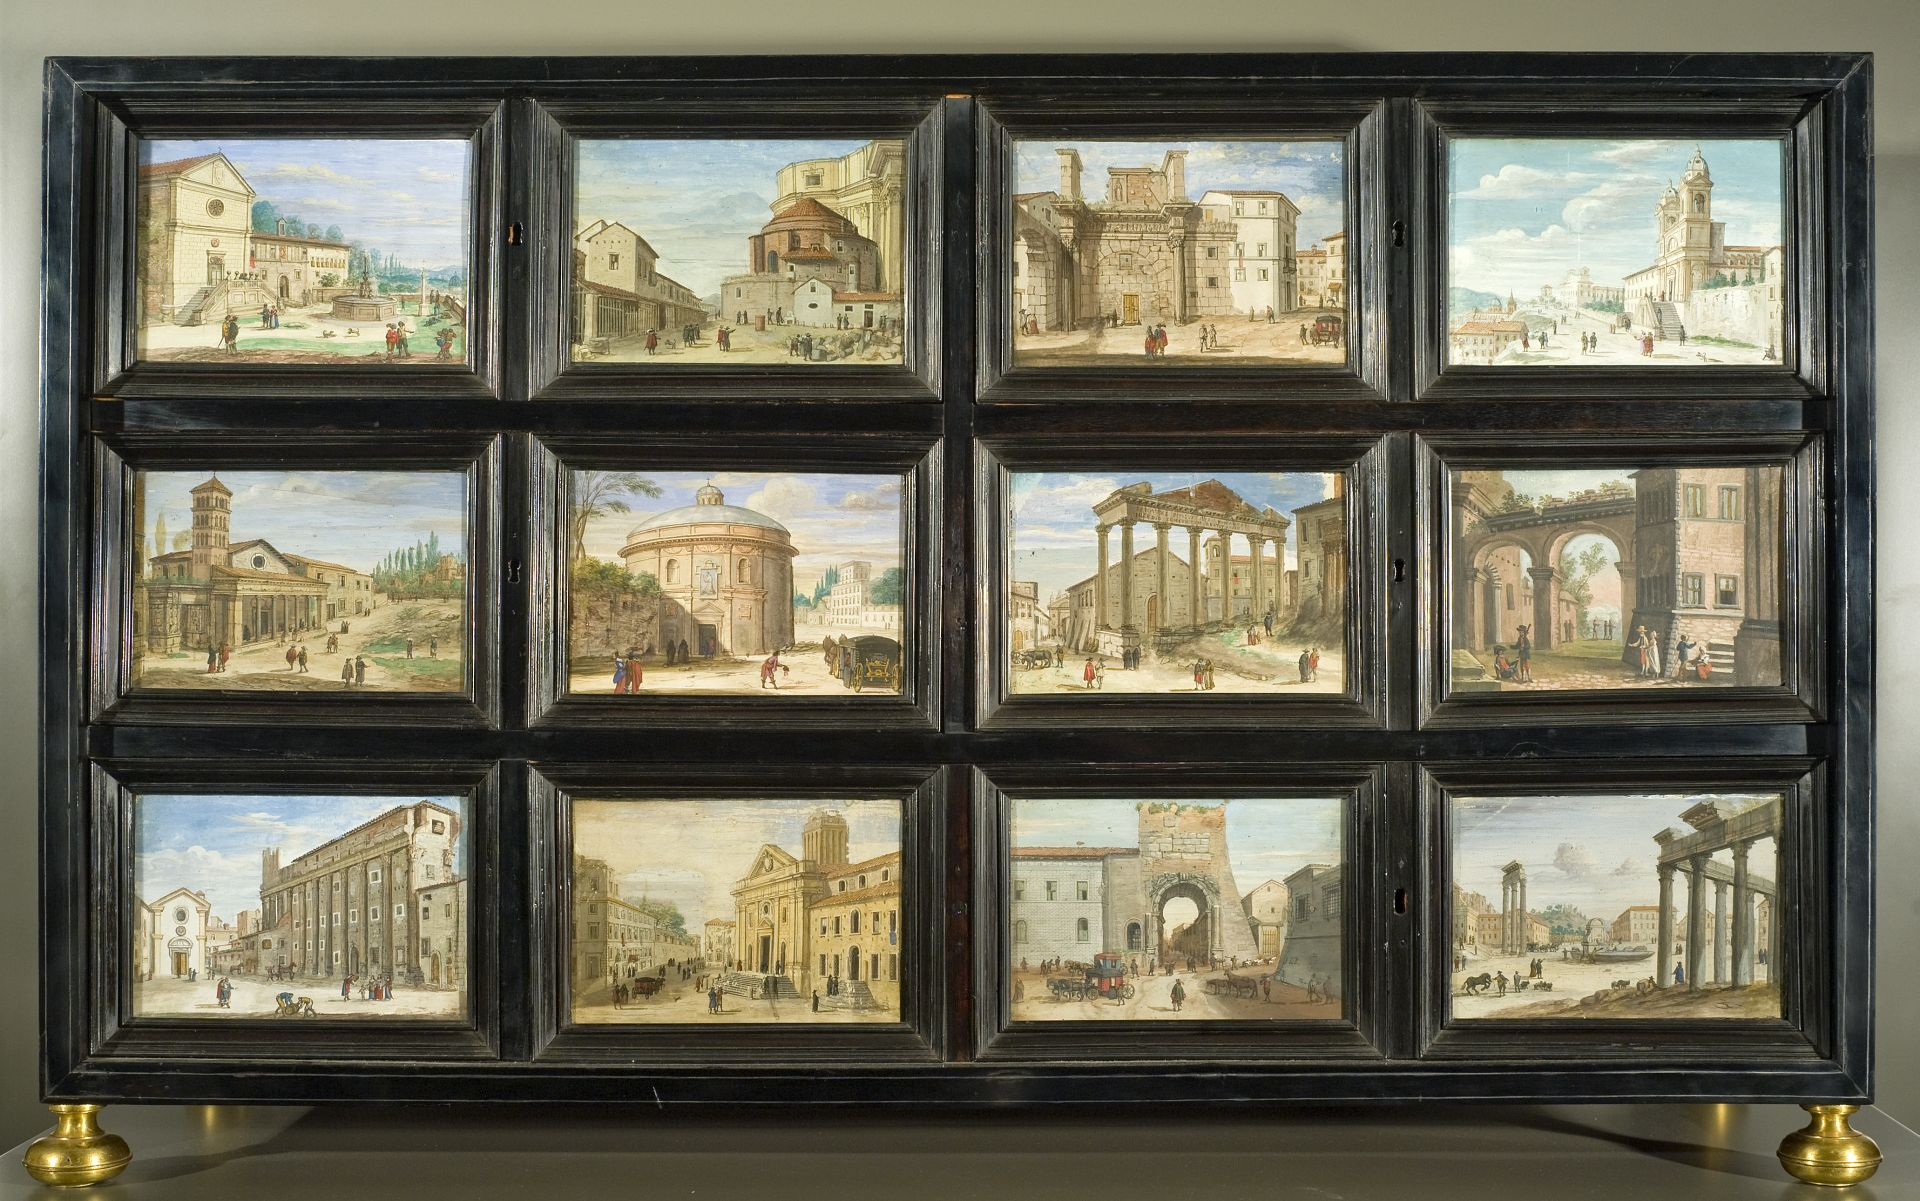
\includegraphics[scale=0.4]{Vedute_di_Roma_1.jpg}}
				\captionof{figure}{Vedute di Roma.}
			\end{minipage}
			\hfill
			\begin{minipage}{0.4\linewidth}
				\zoombox{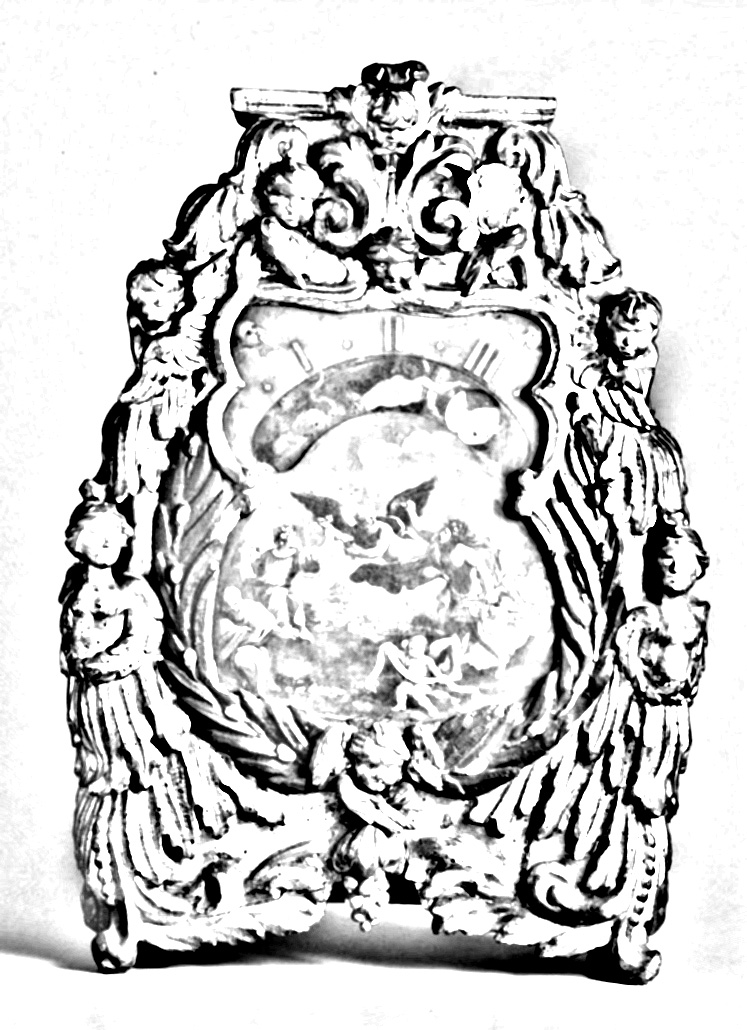
\includegraphics[scale=0.2]{Orologio_notturno.jpg}}
				\captionof{figure}{Orologio notturno.}
			\end{minipage}
		\end{minipage}
	\end{frame}
	
	\subsection{Scacciani Antonio - Vassoio - Rosa}
	\begin{frame}{\numcirc{7} Sottoporre all'attenzione dei visitatori il piatto decorato con la Rosa di Pesaro}
		\begin{itemize}
			\item Mostrare il \textbf{Piatto della bottega pesarese} con \textbf{decoro della Rosa di Pesaro} il cui motivo è tipico della nostra zona.\par \bigskip
			\begin{minipage}{\linewidth}
				\centering
				\zoombox{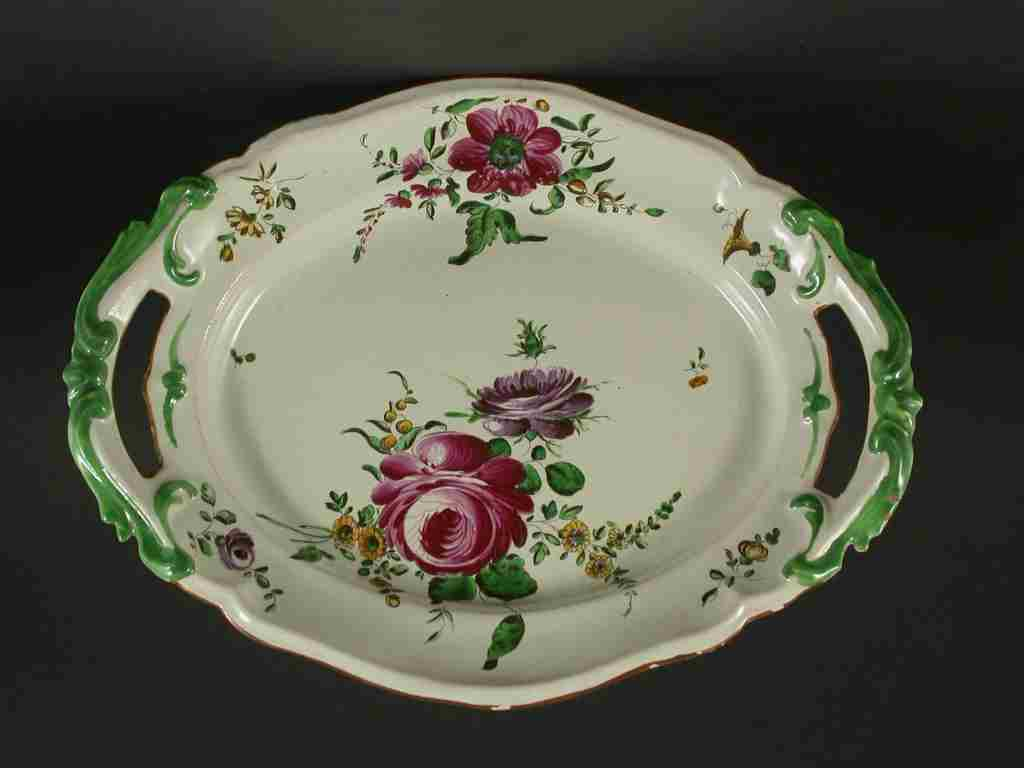
\includegraphics[scale=0.7]{Scacciani_Antonio-Vassoio-Rosa.jpg}}
				\captionof{figure}{Scacciani Antonio - Vassoio - Rosa.}
			\end{minipage}
		\end{itemize}
	\end{frame}
	
	
	\subsection{Milani Aureliano - Mercato}
	\begin{frame}{\numcirc{8} Far visionare il quadro il Mercato di Aureliano Milani}
		\begin{itemize}
			\item Descrivere il dipinto ad olio \textit{Il Mercato di Aureliano Milani}, che rappresenta una scena di vita quotidiana all'interno di un piccolo borgo abitato, in cui sono visibili esponenti di diversi ceti sociali e i loro relativi mestieri.\par
		\end{itemize}
	\end{frame}
	
	\begin{frame}
		\bigskip
		\begin{minipage}{\linewidth}
			\centering
			\zoombox{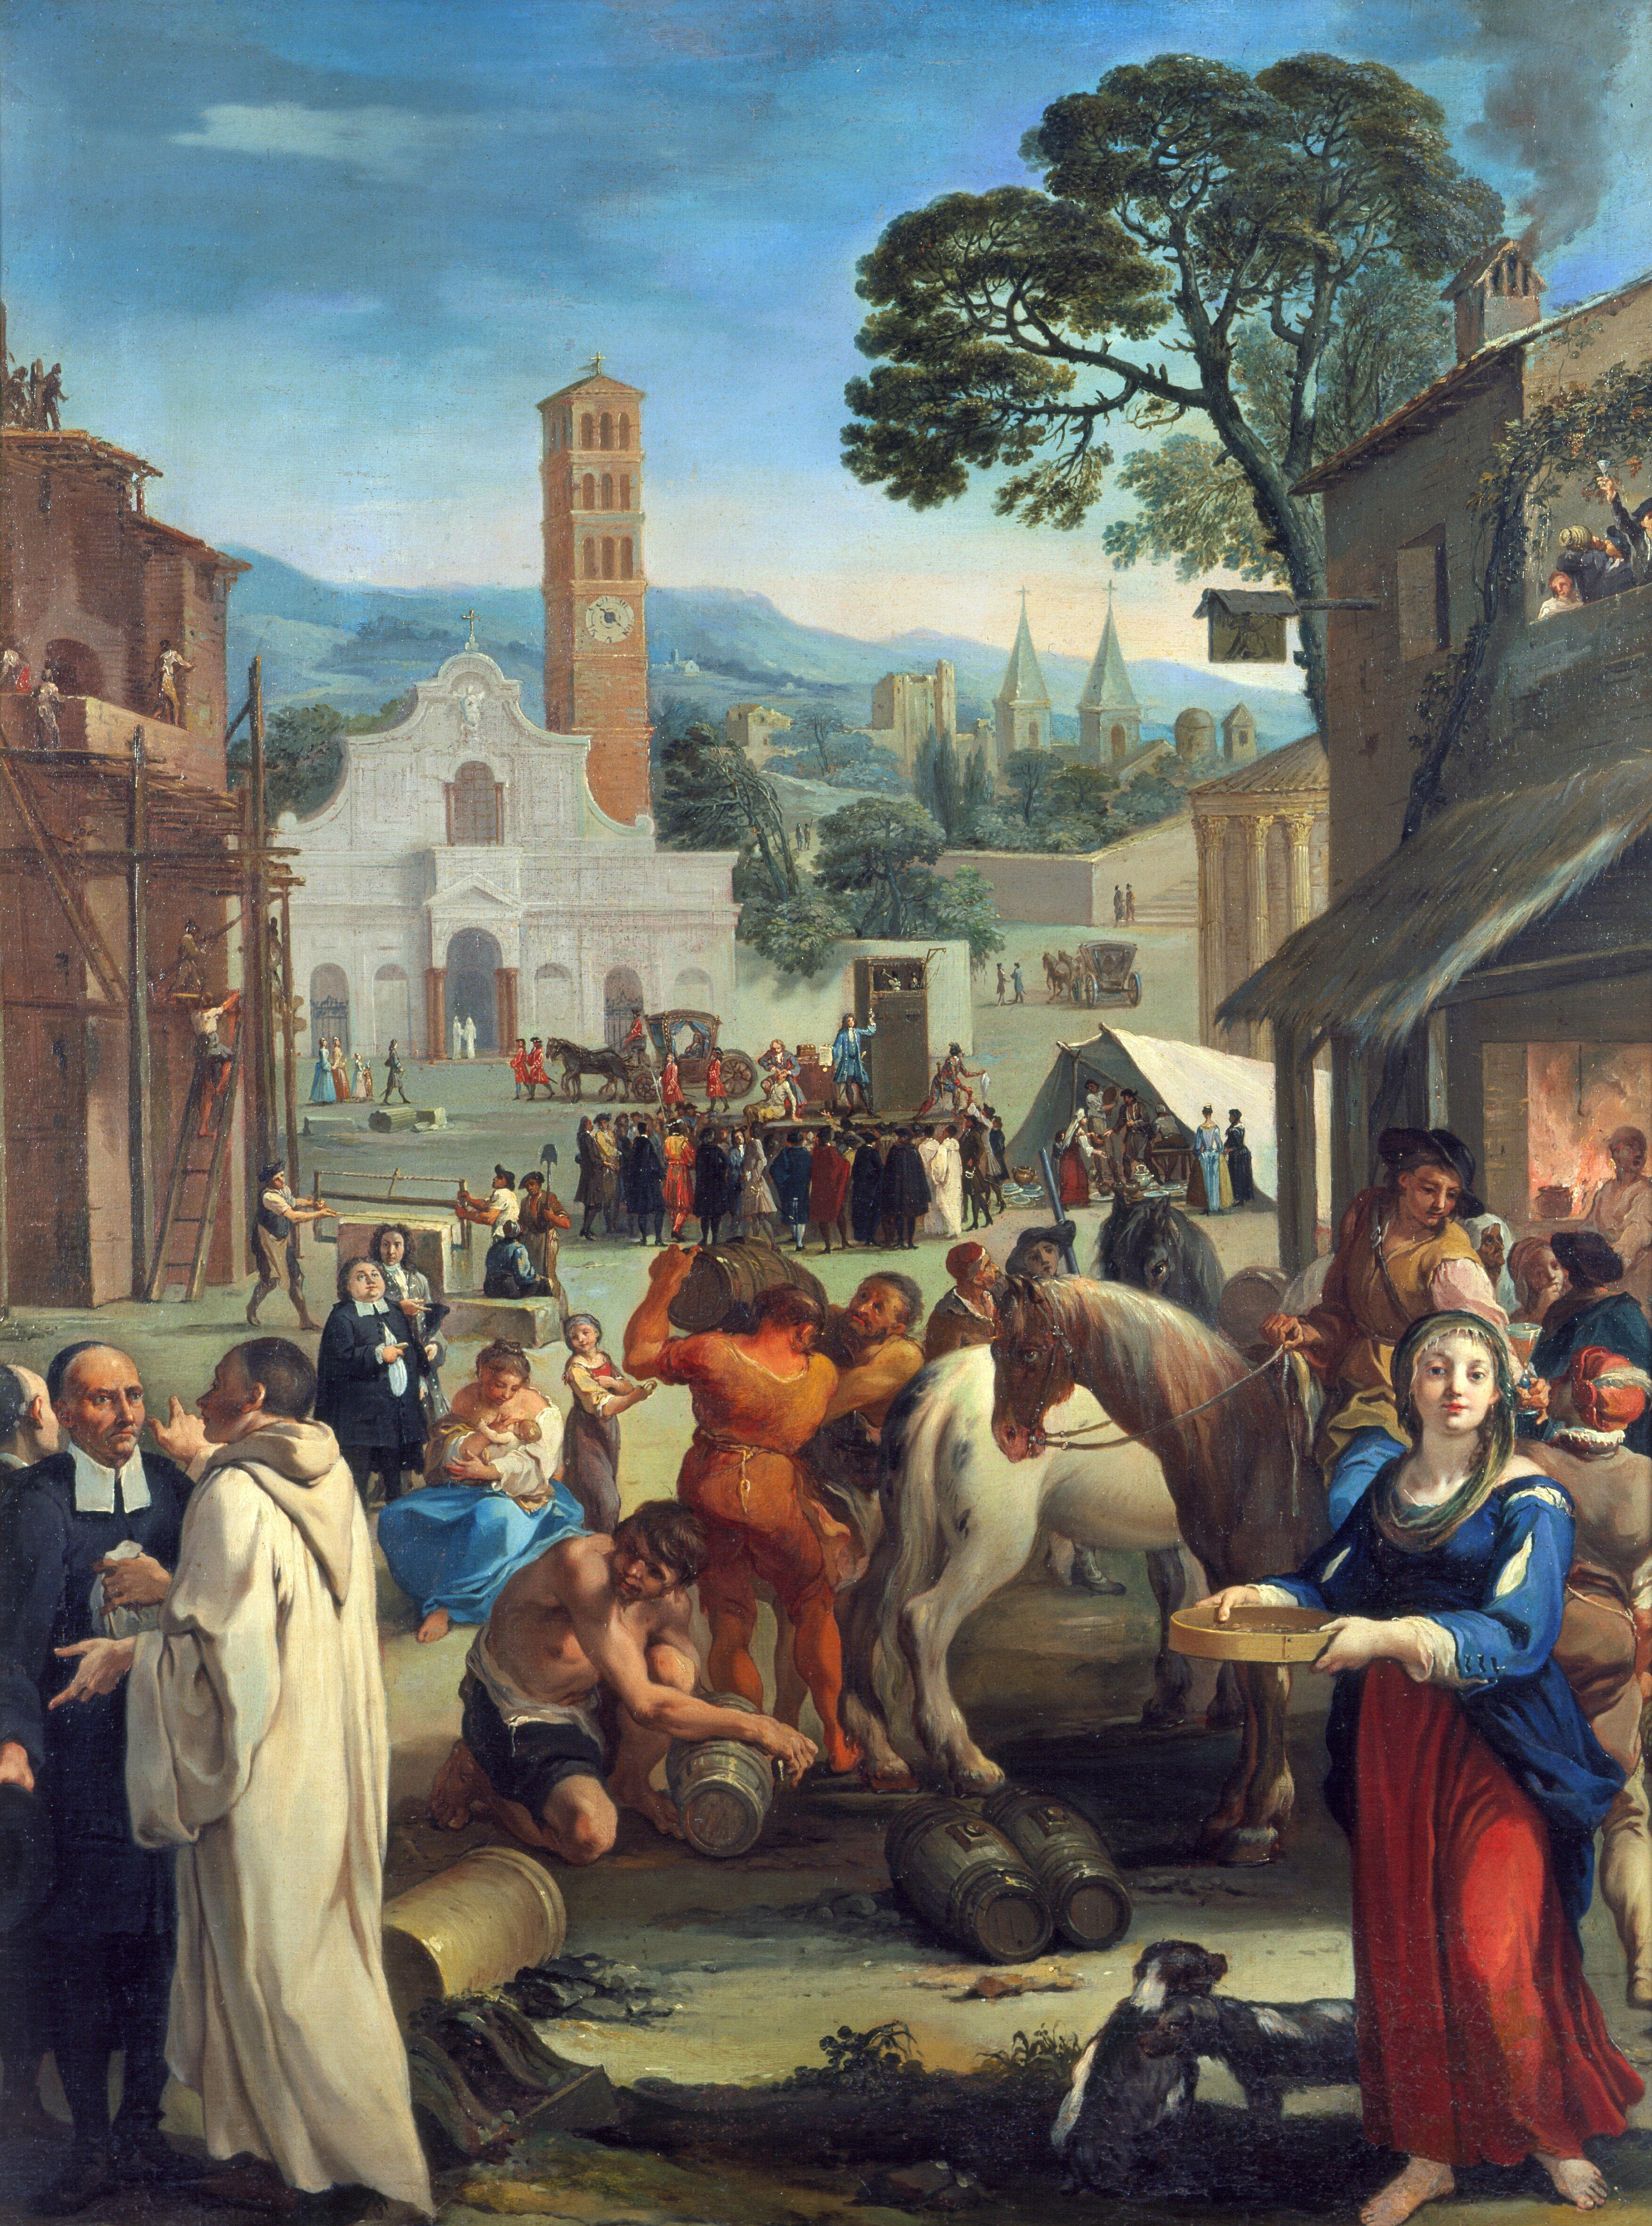
\includegraphics[scale=0.045]{Milani_Aureliano-Mercato.jpg}}
			\captionof{figure}{Milani Aureliano - Mercato.}
		\end{minipage}
	\end{frame}
	
	\subsection{Berentz Christian - Fiori e frutta con bicchieri di cristallo}
	\subsection{Gianlisi Antonio Junior - Trompe l'oeil con sonetto in onore di Eugenio di Savoia e mensola con oggetti}
	\subsection{Gianlisi Antonio Junior - Trompe l'oeil con paesaggio forbici e mensola con oggetti}
	\begin{frame}{\numcirc{9} Far notare le Nature Morte}
		\begin{itemize}
			\item Presentare le \textbf{Nature Morte}, evidenziando la \textbf{frutta} ed i \textbf{calici in vetro}, e come la loro abbondanza fosse anche accompagnata dall'effimera precarietà della loro freschezza, metafora della breve durata della giovinezza.
			 Accompagnare successivamente i bambini davanti ai \textbf{Trompe l'oeil} con il \textbf{Sonetto di Antonio Gianlisi Junior} e il \textbf{Trompe l'oeil} con la \textbf{pipa}, mettendo in risalto i cibi e gli oggetti di uso comune come la \textit{pipa} e i \textbf{savoiardi} che alludono ai Savoia.\par
		\end{itemize}
	\end{frame}

	\begin{frame}
		\bigskip
		\begin{minipage}{\linewidth}
			\centering
			\zoombox{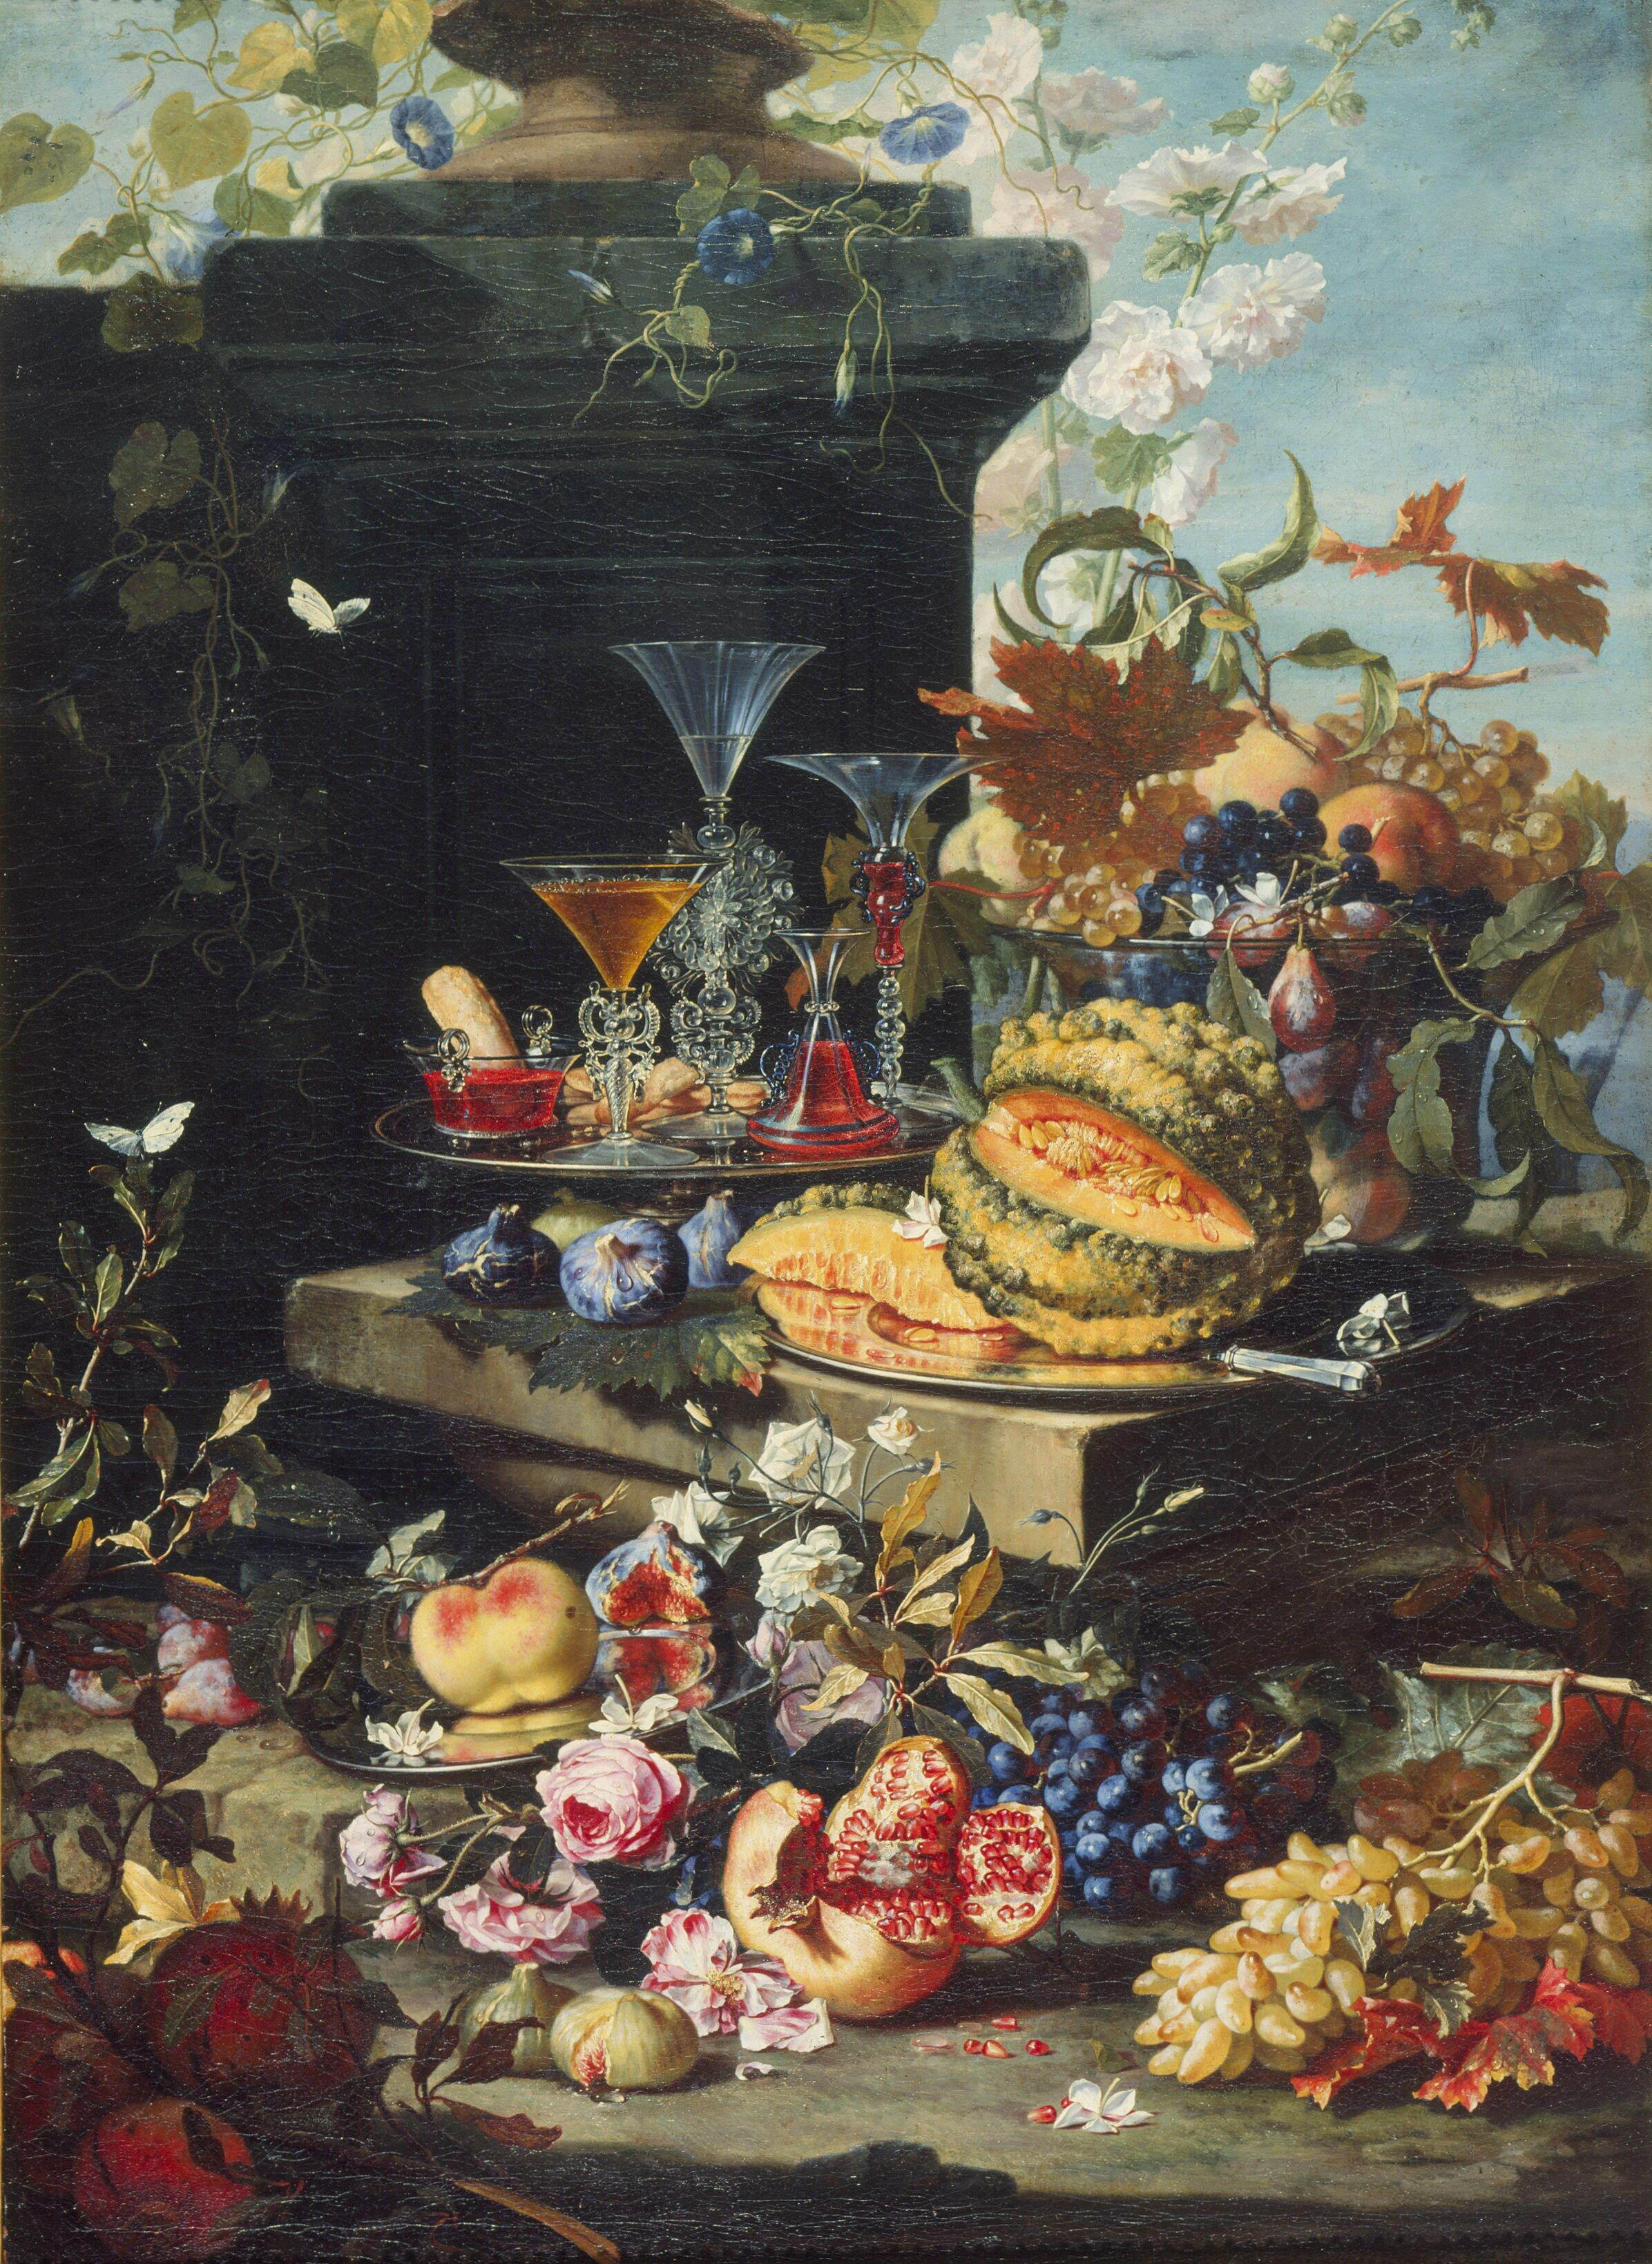
\includegraphics[scale= 0.06]{Berentz_Christian-Fiori_e_frutta_con_bicchieri_di_cristallo.jpg}}
			\captionof{figure}{Berentz Christian - Fiori e frutta con bicchieri di cristallo.}
		\end{minipage}
	\end{frame}

	\begin{frame}
	\bigskip
	\begin{minipage}{\linewidth}
		\centering
		\begin{minipage}[t]{0.4\linewidth}
			\zoombox{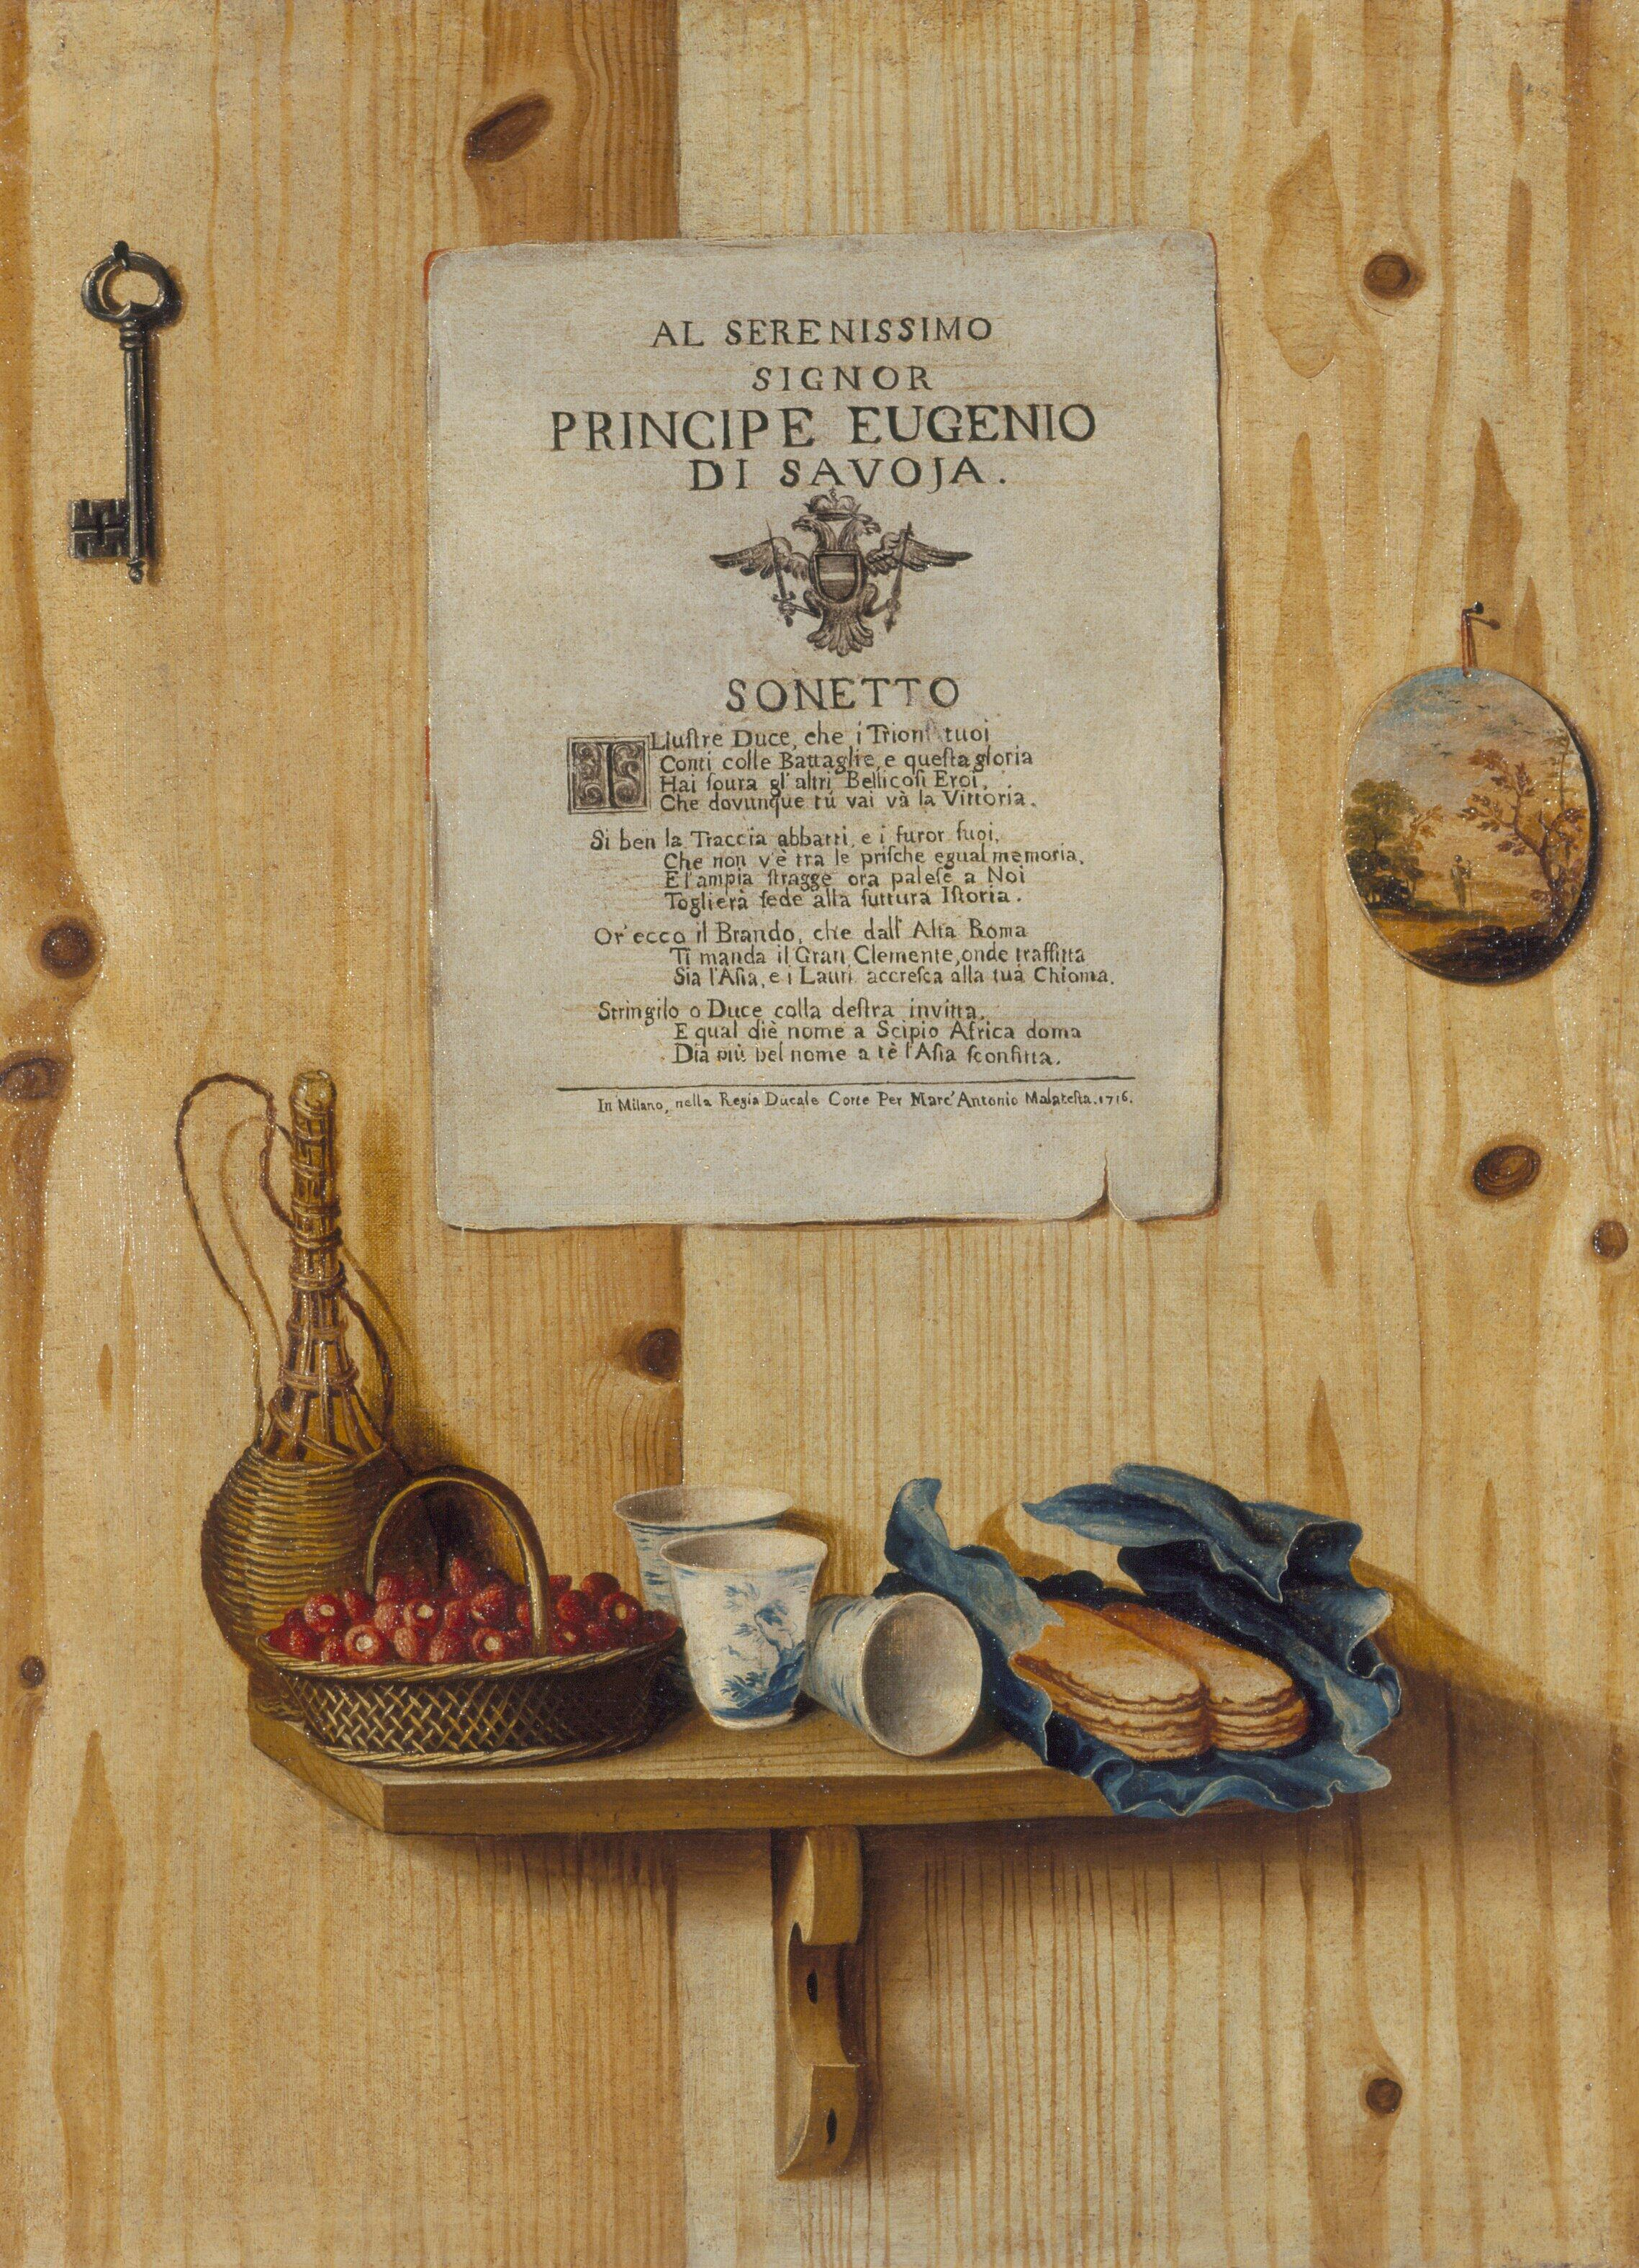
\includegraphics[scale=0.057]{Gianlisi_Antonio_Junior-Trompe_l_oeil_con_sonetto_in_onore_di_Eugenio_di_Savoia_e_mensola_con_oggetti.jpg}}
			\captionof{figure}{Gianlisi Antonio Junior - Trompe l'oeil con sonetto in onore di Eugenio di Savoia e mensola con oggetti.}
		\end{minipage}
		\hfill
		\begin{minipage}[t]{0.4\linewidth}
			\zoombox{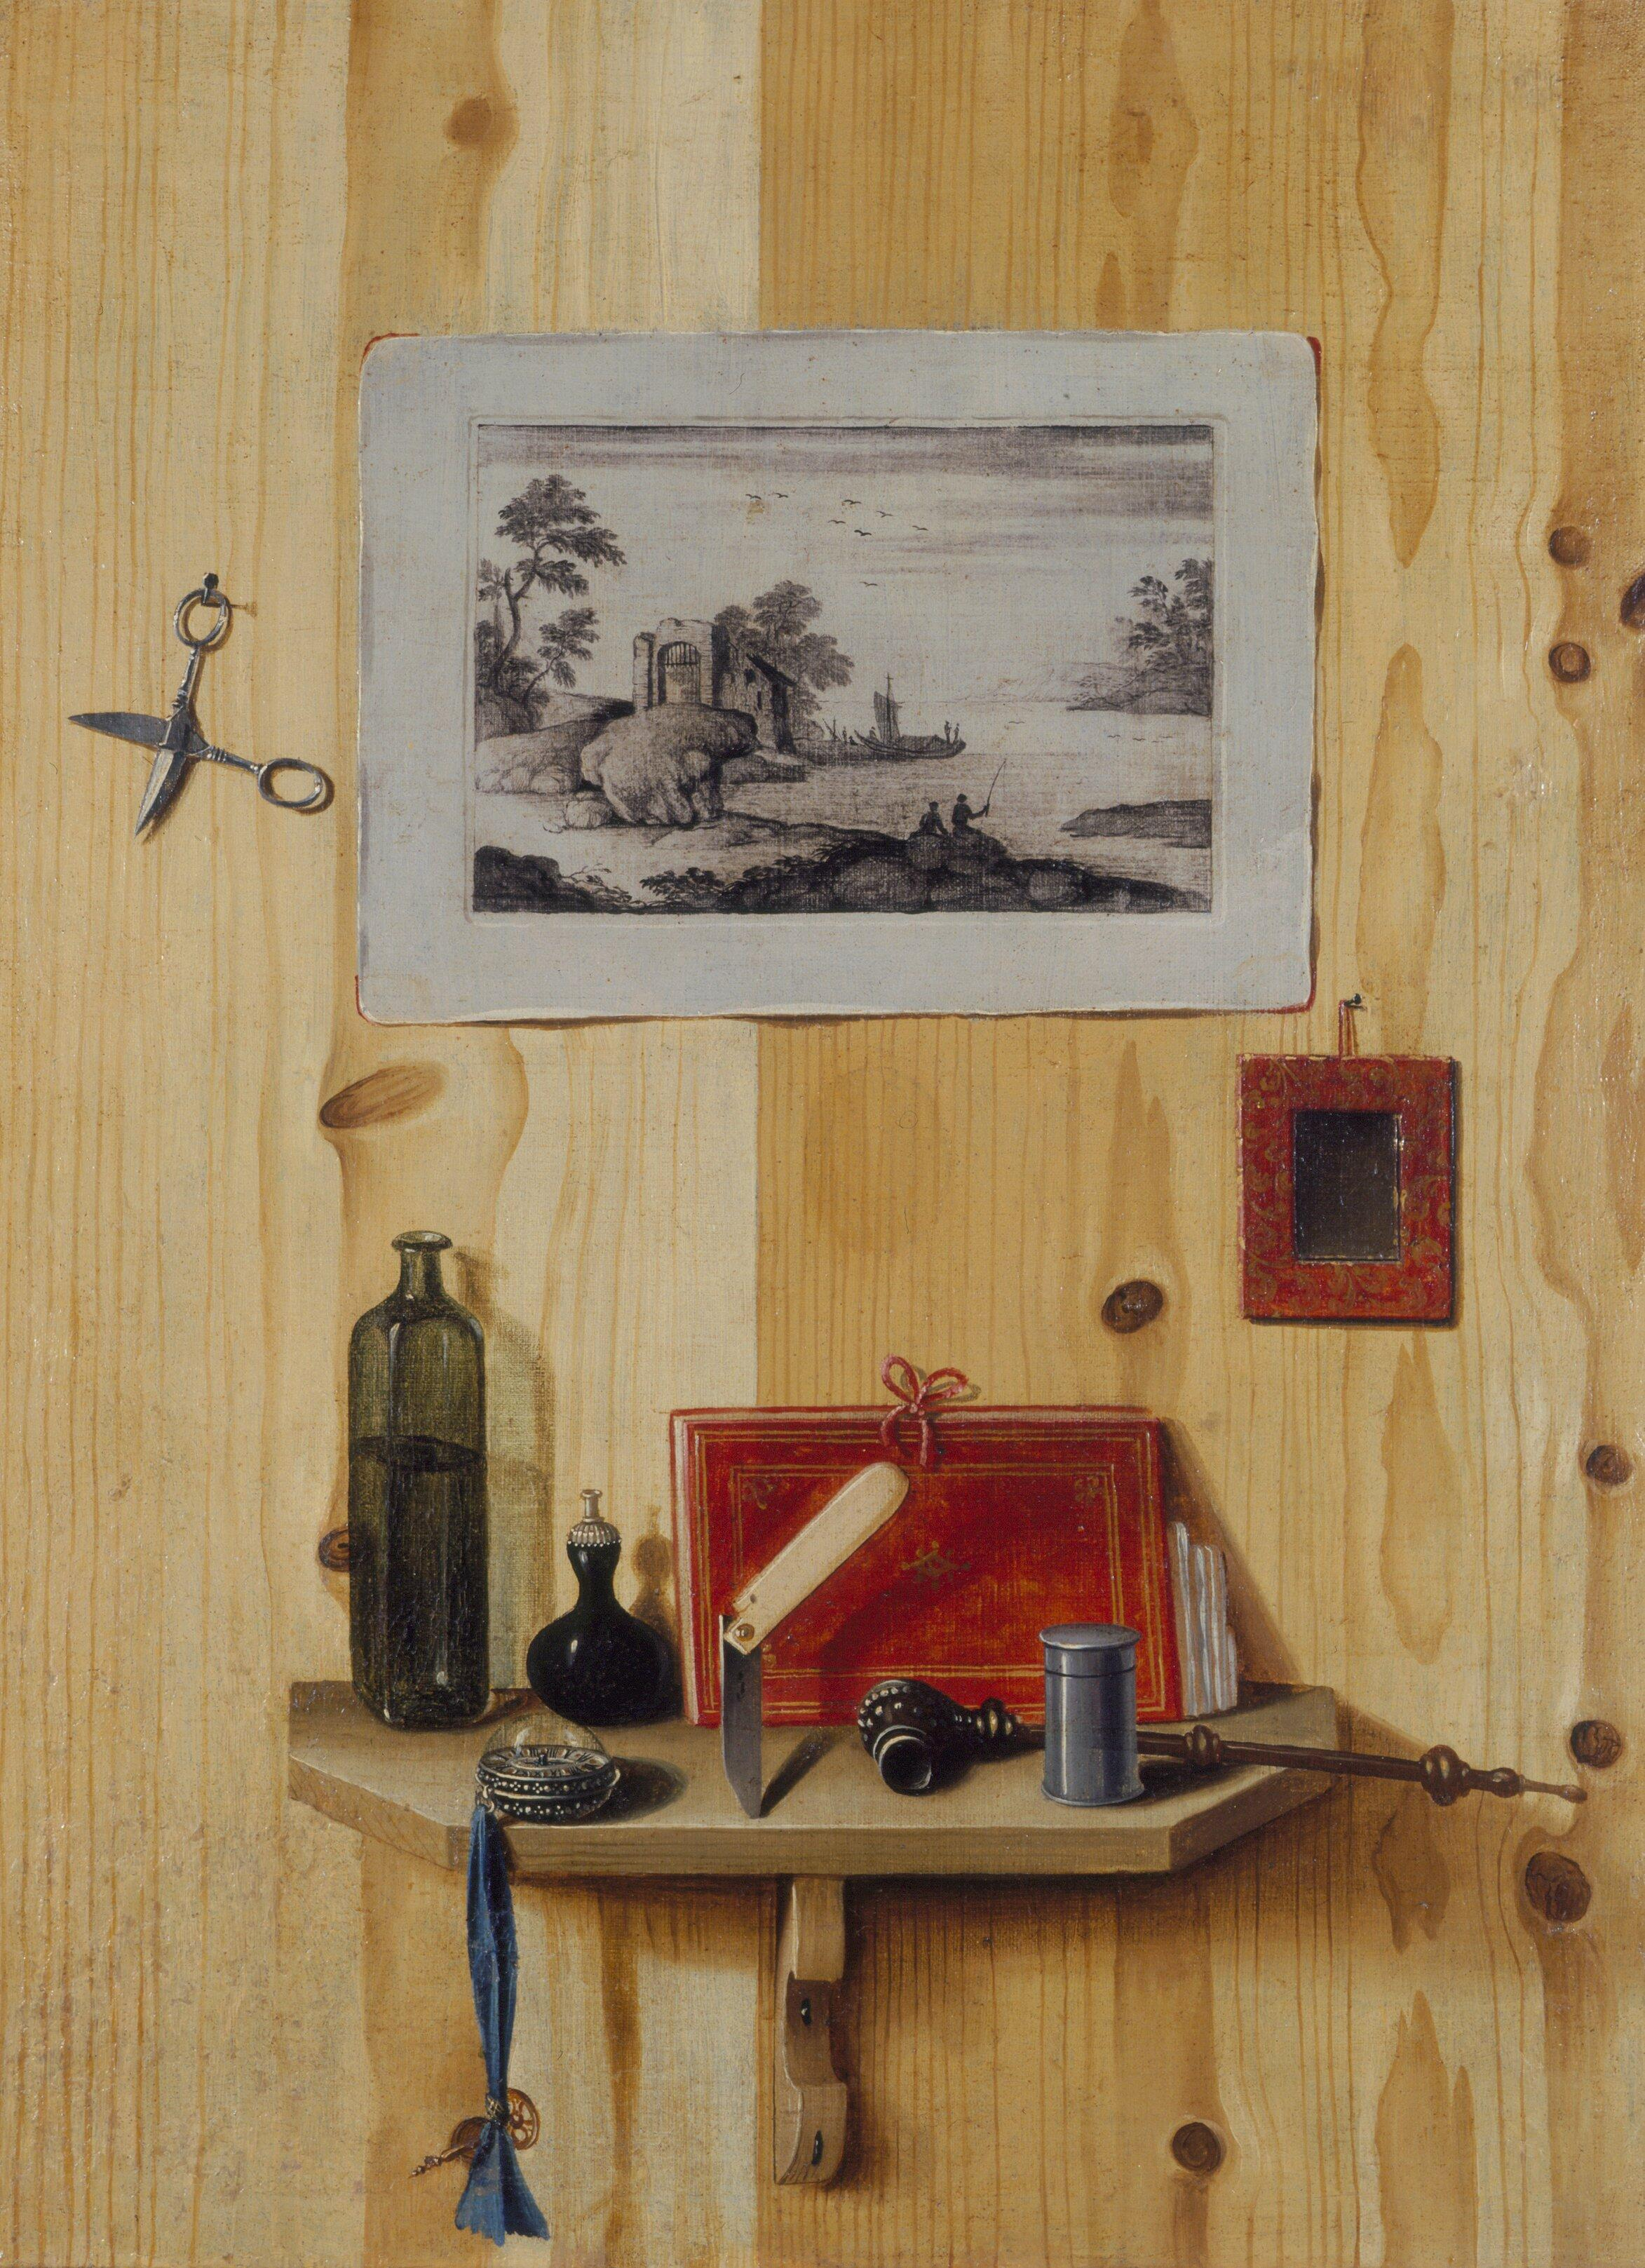
\includegraphics[scale=0.057]{Gianlisi_Antonio_Junior-Trompe_l_oeil_con_paesaggio_forbici_e_mensola_con_oggetti.jpg}}
			\captionof{figure}{Gianlisi Antonio Junior - Trompe l'oeil con paesaggio forbici e mensola con oggetti.}
		\end{minipage}
	\end{minipage}
	\end{frame}
	
	\subsection{Realfonzo Tommaso - Natura morta con dolci frutta uova e formaggi}
	\subsection{Gessi Giovan Francesco - Morte di Adone}
	\begin{frame}{\numcirc{10} Mettere in evidenza dipinti contenenti particolari che possono attirare l'attenzione dei bambini}
		\begin{itemize}
			\item Indicare ai piccoli i dipinti contenenti particolari che possono attirare la loro attenzione, come per esempio \textbf{le uova, i salami ed i limoni} nel dipinto \textit{Dispensa con dolci, uova, salame, formaggi, ghiacciata e canestro di limoni} oppure il dettaglio del \textbf{cinghiale} presente nella \textbf{Morte di Adone}, piccolo dettaglio che ci svela come il protagonista sia tragicamente morto durante una battuta di caccia.\par
		\end{itemize}
	\end{frame}
	
	\begin{frame}
		\bigskip
		\begin{minipage}{\linewidth}
			\centering
			\begin{minipage}[t]{0.4\linewidth}
			\zoombox{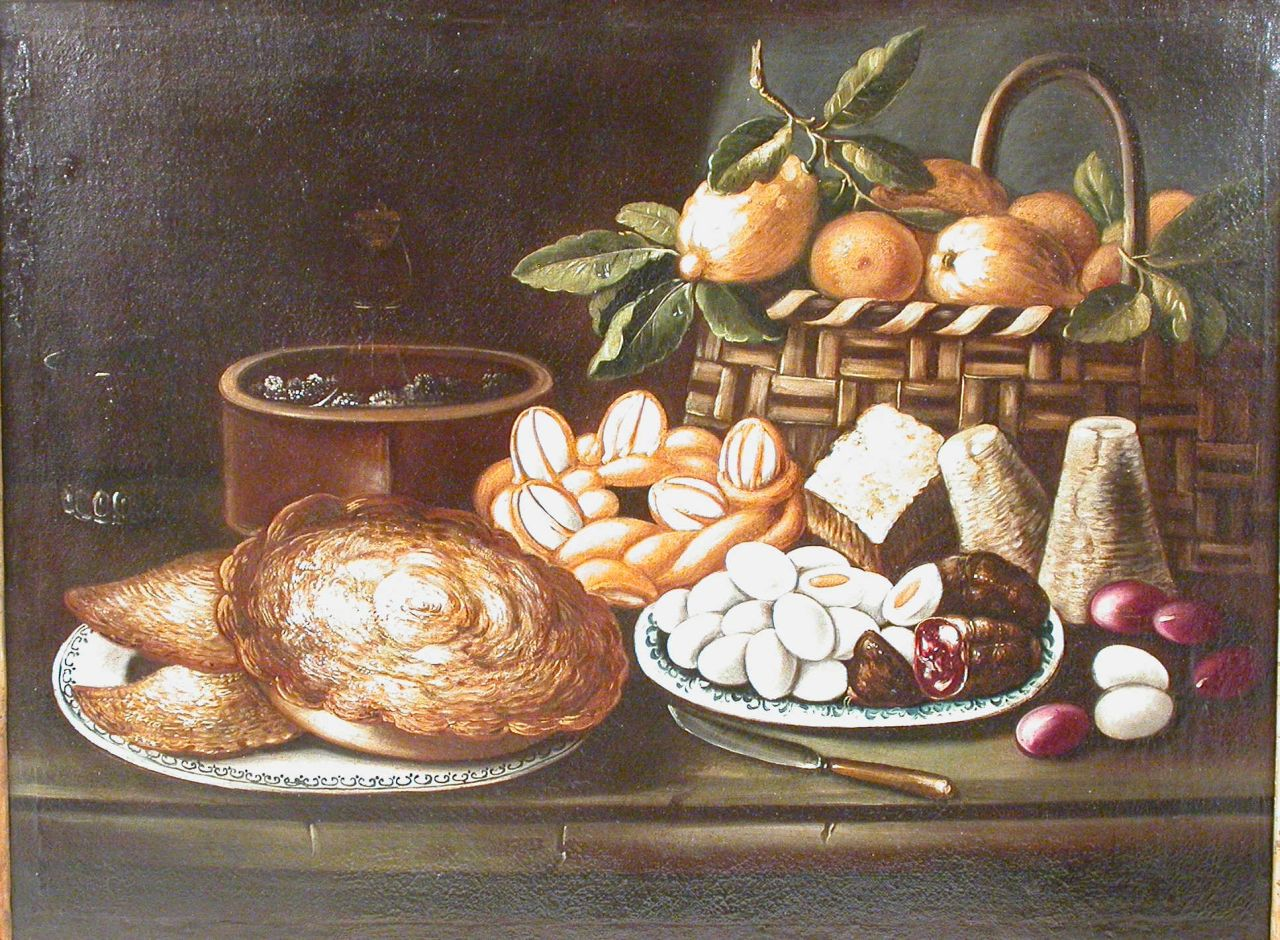
\includegraphics[scale=0.6]{Realfonzo_Tommaso-Natura_morta_con_dolci_frutta_uova_e_formaggi.jpg}}
			\captionof{figure}{Realfonzo Tommaso - Natura morta con dolci frutta uova e formaggi.}
			\end{minipage}
			\hfill
			\begin{minipage}[t]{0.5\linewidth}
				\zoombox{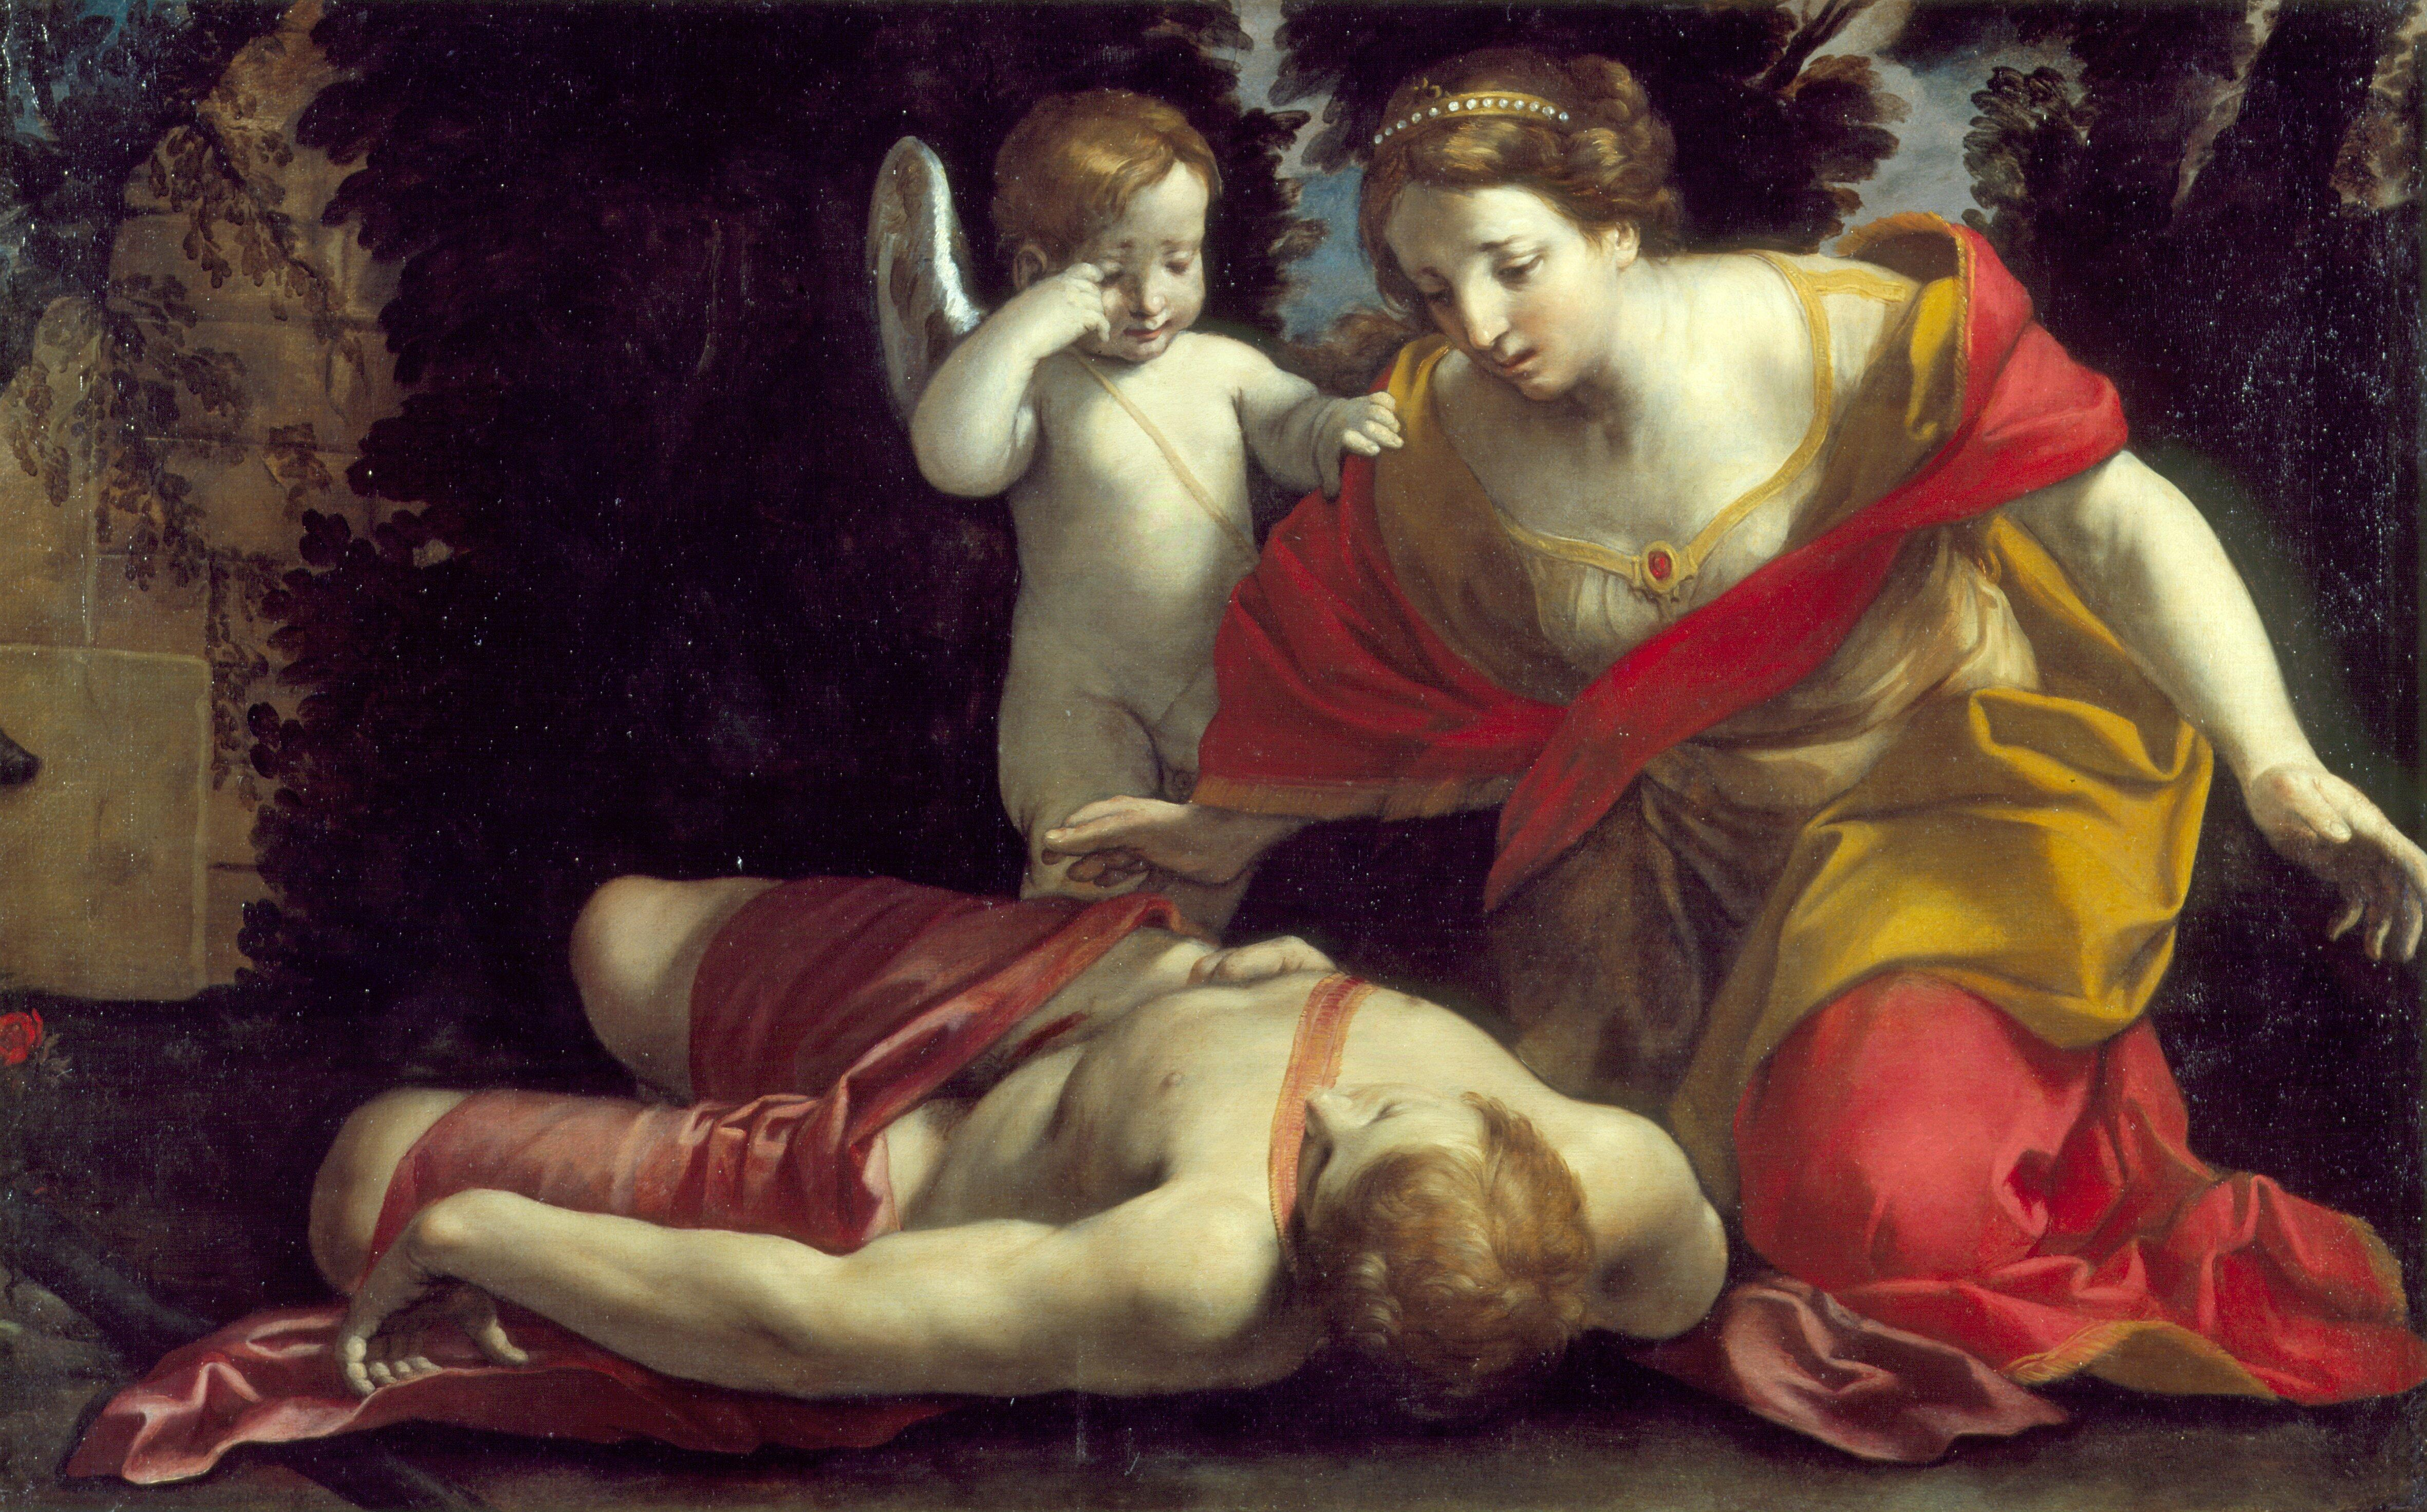
\includegraphics[scale=0.045]{Gessi_Giovan_Francesco-Morte_di_Adone.jpg}}
				\captionof{figure}{Gessi Giovan Francesco - Morte di Adone.}
			\end{minipage}
		\end{minipage}
	\end{frame}
	
	\begin{frame}{\numcirc{11} Far provare l'esperienza della Sonosfera}
		\begin{itemize}
			\item Questa particolare struttura permette la visione di due spettacoli, che si caratterizzano per l'immersione profonda nell'ascolto sonoro.\\
			 Il primo di questi spettacoli è:"Frammenti di Estinzione nell'Orologio Climatico"e permette a chi lo osserva di comprendere quanto sia importante accelerare il processo per la transizione alle energie verdi e quanto sia necessario preservare la Natura che ci circonda: tutto questo attraverso l'ascolto dei suoni delle Foreste Equatoriali, registrati durante i suoi viaggi dal Professore del Conservatorio Rossini Davide Monacchi.\\
			  Il secondo spettacolo è invece dedicato ad apprendere e scoprire l'arte del cellebre pittore Raffaello, in maniera del tutto innovativa, poiché è possibile in questa struttura visionare anche i bozzetti tracciati con la matita sanguigna, in preparazione ai suoi affreschi nella Sala della Signatura ai Musei Vaticani. L'ascolto di musiche contemporanee a Raffaello, permette di immergersi totalmente nella visione delle sue opere e del contesto che le ha prodotte. La sala per l'ascolto è però buia e il suono può risultare alto per i più giovani spettatori che potrebbero spaventarsi; (esperienza più volte verificata di persona)si consiglia quindi la vsione alle classi di medie o superiori.
		\end{itemize}
	\end{frame}

\section{Fonti e Licenza}
\begin{frame}{Fonti e Licenza}
	Le informazioni riportate sono tratte dalle audio-guide dei Musei Civici.
	
	\vspace*{\fill}
	% Print license shield
	\doclicenseThis
\end{frame}	
\end{document}